\documentclass[UTF8,a4paper,12pt]{ctexrep}

\usepackage{geometry}
\usepackage{graphicx}
\usepackage{booktabs}
\usepackage{longtable}
\usepackage{tabularx}
\usepackage{array}
\usepackage{amsmath}
\usepackage{amssymb}
\usepackage{caption}
\usepackage{subcaption}
\usepackage{float}
\usepackage{enumitem}
\usepackage{xcolor}
\usepackage{listings}
\usepackage[hidelinks]{hyperref}

\geometry{left=2.7cm,right=2.7cm,top=2.8cm,bottom=2.8cm}
\setlength{\parindent}{2em}
\setlength{\parskip}{0.25em}
\renewcommand{\arraystretch}{1.18}
\graphicspath{{figures/}}
\sloppy

\lstdefinestyle{pythoncode}{
  language=Python,
  basicstyle=\ttfamily\small,
  keywordstyle=\color{blue!60!black},
  commentstyle=\color{green!40!black},
  stringstyle=\color{red!50!black},
  showstringspaces=false,
  breaklines=true,
  frame=single,
  columns=fullflexible,
  keepspaces=true,
  tabsize=4
}
\lstdefinestyle{bashcode}{
  basicstyle=\ttfamily\small,
  keywordstyle=\color{blue!60!black},
  commentstyle=\color{green!40!black},
  showstringspaces=false,
  breaklines=true,
  frame=single,
  columns=fullflexible,
  keepspaces=true
}
\lstset{style=pythoncode}

\newcommand{\Mw}{M_{\mathrm{w}}}
\newcommand{\dd}{\,\mathrm{d}}
\newcommand{\loss}{\mathcal{L}}

\begin{document}

\newgeometry{left=2.45cm,right=2.45cm,top=1.15cm,bottom=1.20cm}
\begin{titlepage}
  \thispagestyle{empty}
  \centering
  \vspace*{0.05cm}
  \IfFileExists{figures/pku_logo_wordmark.png}{
\includegraphics[width=8.7cm]{pku_logo_wordmark.png}\par}{\vspace*{1cm}}
  \vspace{2.70cm}

  {\zihao{0}\heiti 研究报告\par}
  \vspace{1.05cm}

  \setlength{\tabcolsep}{0pt}
  \begin{tabular}{@{}p{2.35cm}p{10.65cm}@{}}
    {\zihao{3}\songti 题目：} &
    \begin{minipage}[t]{10.65cm}
      \centering
      {\zihao{3}\songti 余震预测技术国际大赛算法研究与工程实现报告}\\[-0.15cm]
      \rule{10.65cm}{0.6pt}
    \end{minipage}
  \end{tabular}

  \vspace{3.60cm}

  \begin{tabular}{@{}p{2.35cm}p{10.65cm}@{}}
    {\zihao{4}\songti 课程：} & \underline{\makebox[10.65cm][c]{\zihao{4}\songti 人工智能导论}} \\[1.25em]
    {\zihao{4}\songti 姓名：} & \underline{\makebox[10.65cm][c]{\zihao{4}\songti 宁业栋}} \\[1.25em]
    {\zihao{4}\songti 学号：} & \underline{\makebox[10.65cm][c]{\zihao{4}\songti 2501220176}} \\[1.25em]
    {\zihao{4}\songti 组别：} & \underline{\makebox[10.65cm][c]{\zihao{4}\songti 个人项目}} \\[1.25em]
    {\zihao{4}\songti 项目：} & \underline{\makebox[10.65cm][c]{\zihao{4}\songti 阿里云天池余震预测技术国际大赛}} \\[1.25em]
  \end{tabular}

  \vfill
  {\zihao{3}\songti 二〇二六年五月\par}
\end{titlepage}
\restoregeometry

\pagenumbering{Roman}
\chapter*{摘要}
\addcontentsline{toc}{chapter}{摘要}

余震预测是地震应急响应中的高价值问题。强震发生后的前数小时至数天，余震序列会快速释放关于断层尺度、应力调整和构造背景的信息；如何利用这一早期观测窗口预测未来最大余震的震级与发生时间，是地震学经验规律、机器学习建模和工程化推理共同作用的复杂任务。本文围绕阿里云天池“余震预测技术国际大赛”构建了一套可复现的端到端算法工程，面向全球浅源强震样本，预测震后未来窗口内最大余震震级与时间差。

本研究使用 USGS 全球地震目录构建主震--余震样本，结合 Peter Bird 2002 全球板块边界数据与 Global CMT 震源机制解，形成包含 4704 条主震样本、82 列高级特征的建模数据集。特征工程部分融合 Gutenberg--Richter 定律、大森--宇津余震衰减、Båth's Law、地震生产率指数、空间各向异性、板块边界距离、震源机制类型和早期能量释放过程。模型部分以 LightGBM 与 XGBoost 为稳定主线，引入时间序列交叉验证、时间目标 \(\log(1+t)\) 变换、预测偏晚非对称惩罚和 OOF 融合；同时实现 Transformer 与有向时空因果 ST-GNN 作为可选深度模型扩展。

实验结果显示，在 5 折 TimeSeriesSplit 验证中，XGBoost 的平均时间 RMSE 为 2.454，LightGBM 非对称时间目标的平均震级 RMSE 为 1.381，树模型 OOF 融合后的震级 RMSE 为 1.370。最终一键流程生成 20 条比赛验证序列的提交文件，包含 \texttt{mainshock\_id}、\texttt{predicted\_max\_mag} 与 \texttt{predicted\_time\_to\_max} 三列，无缺失值且预测时间均非负。本文最后总结了当前方案的工程优势与局限，并讨论低震级完整目录、区域构造分层建模和深度时空模型进一步提升的方向。

\noindent\textbf{关键词：} 余震预测；Gutenberg--Richter 定律；Omori--Utsu 定律；Global CMT；LightGBM；XGBoost；Transformer；ST-GNN；时间序列交叉验证

\tableofcontents
\clearpage
\pagenumbering{arabic}

\chapter{引言}

\section{研究背景}
大震之后的余震活动不仅影响救援安全、基础设施恢复和公众避险决策，也为理解主震破裂尺度和区域应力调整提供了重要线索。经验地震学表明，余震频率通常随时间按幂律衰减，震级频度服从 Gutenberg--Richter 关系，最大余震与主震震级差值又呈现 Båth's Law 所描述的统计规律。然而，这些规律在不同构造环境、震源机制与观测完整性条件下会发生显著变化，单一经验公式很难覆盖全球浅源强震的复杂情形。

本项目的比赛任务要求：针对全球范围内发生的浅源强震，在主震发生后早期观测窗口内获取地震序列、构造背景和震源机制信息，预测未来特定时间段内最大余震的震级和发生时间。该任务存在三个核心难点。第一，目标分布高度零膨胀与长尾并存，大量样本未来窗口无显著余震，而少数强余震样本决定了风险上限。第二，不同构造区的余震生产率差异显著，俯冲带、走滑断层和板内地震的统计行为并不一致。第三，真实线上评测天然按时间推进，若使用随机划分会产生未来信息泄漏，导致离线指标虚高。

\section{研究目标}
本文目标不是仅给出单个模型，而是建立一套“数据--特征--模型--评估--提交”闭环工程。具体包括：
\begin{enumerate}[label=\arabic*.]
  \item 构建全球浅源强震主震--余震样本，并生成与比赛提交逻辑一致的训练标签；
  \item 融合地震学先验与机器学习特征，包括 G-R b 值、大森--宇津参数、Båth 缺口、空间各向异性、板块边界和 Global CMT 震源机制；
  \item 建立严格时间序列验证体系，避免未来数据穿越；
  \item 训练 LightGBM、XGBoost 基线模型，并以 OOF 方式搜索融合权重；
  \item 实现 Transformer 和 ST-GNN 深度模型接口，为后续深度时空建模预留可复现路径；
  \item 输出可一键运行的比赛推理流水线和标准提交文件。
\end{enumerate}

\section{工程流水线概览}
项目总体流程如图\ref{fig:pipeline}所示。原始数据层包括 USGS 地震目录、PB2002 板块边界和 Global CMT 震源机制目录；特征层将早期余震序列转化为统计、物理和构造特征；模型层以树模型为主线，并保留深度序列模型；推理层对每个测试序列实时提取特征并输出提交格式。

\begin{figure}[H]
  \centering
  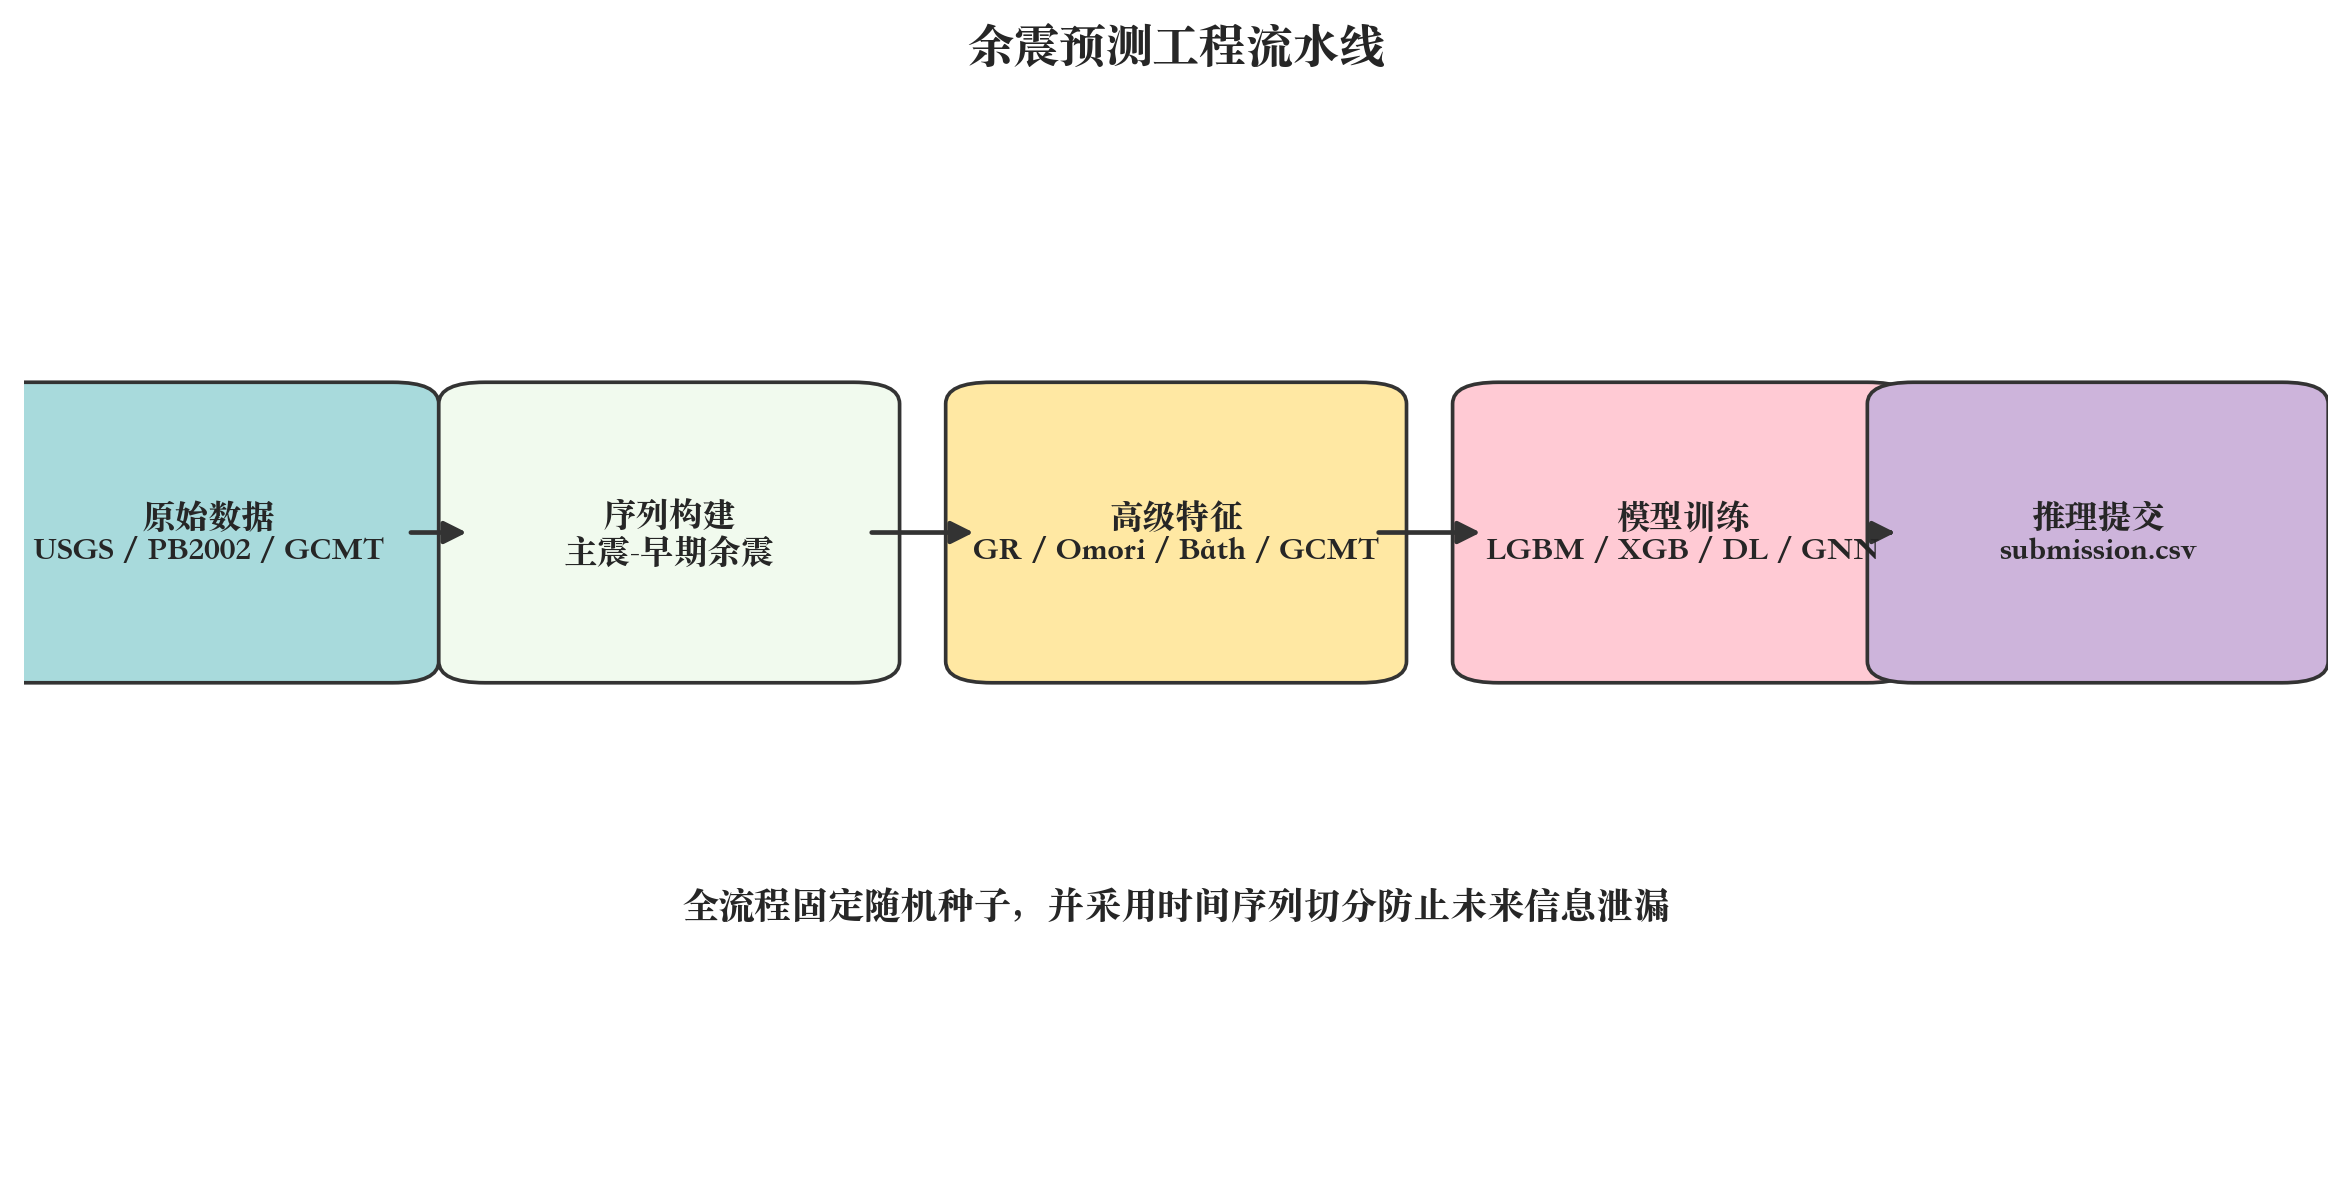
\includegraphics[width=0.96\textwidth]{pipeline_flow.png}
  \caption{余震预测工程流水线}
  \label{fig:pipeline}
\end{figure}

\chapter{数据集与样本构建}

\section{数据源}
本项目使用多源地震学数据。USGS 地震目录提供事件时间、经纬度、深度和震级，是主震识别与早期余震序列重建的基础；PB2002 板块边界提供最近边界距离和边界类型；Global CMT 提供震源机制解，刻画断层滑动方式。主要数据源见表\ref{tab:data_sources}。

\begin{table}[H]
  \centering
  \caption{数据源与用途}
  \label{tab:data_sources}
  \begingroup
\footnotesize
\setlength{\tabcolsep}{4pt}
\begin{tabular}{p{0.24\textwidth}p{0.36\textwidth}p{0.30\textwidth}}
\toprule
数据源 & 路径 & 用途 \\
\midrule
USGS Mw>=4.0 浅源目录 & USGS\_Mw4.0\_Depth70\_1970-2023.csv & 重建主震后 3 天早期余震序列 \\
USGS Mw>=6.0 主震目录 & USGS\_Mw6.0\_Depth70\_1970-2023.csv & 确定强震主震样本 \\
PB2002 板块边界 & PB2002\_boundaries.json & 最近板块边界距离与边界类型 \\
Global CMT & GlobalCMT\_1976-2024.csv & 震源机制 strike/dip/rake 与断层类型 \\
比赛验证序列 & data/test\_sequences/*\_eq.csv & 20 条单序列推理验证 \\
\bottomrule
\end{tabular}
\endgroup

\end{table}

处理后的样本规模见表\ref{tab:dataset_summary}。当前高级特征表包含 4704 条主震样本、82 列字段，其中训练脚本自动筛选 74 个数值特征进入树模型。20 条比赛验证序列已经通过推理脚本生成提交文件。

\begin{table}[H]
  \centering
  \caption{样本与特征规模}
  \label{tab:dataset_summary}
  \begingroup
\footnotesize
\setlength{\tabcolsep}{4pt}
\begin{tabular}{lr}
\toprule
统计项 & 数值 \\
\midrule
主震样本数 & 4711 \\
高级特征列数 & 83 \\
模型输入特征数 & 94 \\
目标最大余震非零样本 & 2981 \\
目标时间非零样本 & 2981 \\
提交序列数 & 20 \\
\bottomrule
\end{tabular}
\endgroup

\end{table}

\section{主震--余震样本定义}
设主震发生时刻为 \(t_0\)，震中位置为 \((\phi_0,\lambda_0)\)。本研究以主震后 \(T_{\mathrm{obs}}=3\) 天作为早期观测窗口，以震中半径 \(R=100\) km 作为空间窗口，筛选满足
\[
  0 < t_i-t_0 \le T_{\mathrm{obs}}, \qquad d_i \le R
\]
的事件作为早期余震序列。未来预测目标包括两项：最大余震震级 \(\hat{M}_{\max}\) 与最大余震发生时间差 \(\hat{t}_{\max}\)。当未来窗口内无满足条件的余震时，目标被记录为 0，这也是目标分布零膨胀的主要来源。

图\ref{fig:sample_distribution}展示了主震样本在时间和震级维度上的分布。样本时间跨度为 1970 年至 2023 年，覆盖全球仪器记录较完整的现代时期。震级分布集中在 \(\Mw 6.0\) 附近，较大震级样本数量迅速下降，这符合强震频度随震级增加而指数衰减的基本规律。

\begin{figure}[H]
  \centering
  \begin{subfigure}{0.48\textwidth}
    \centering
    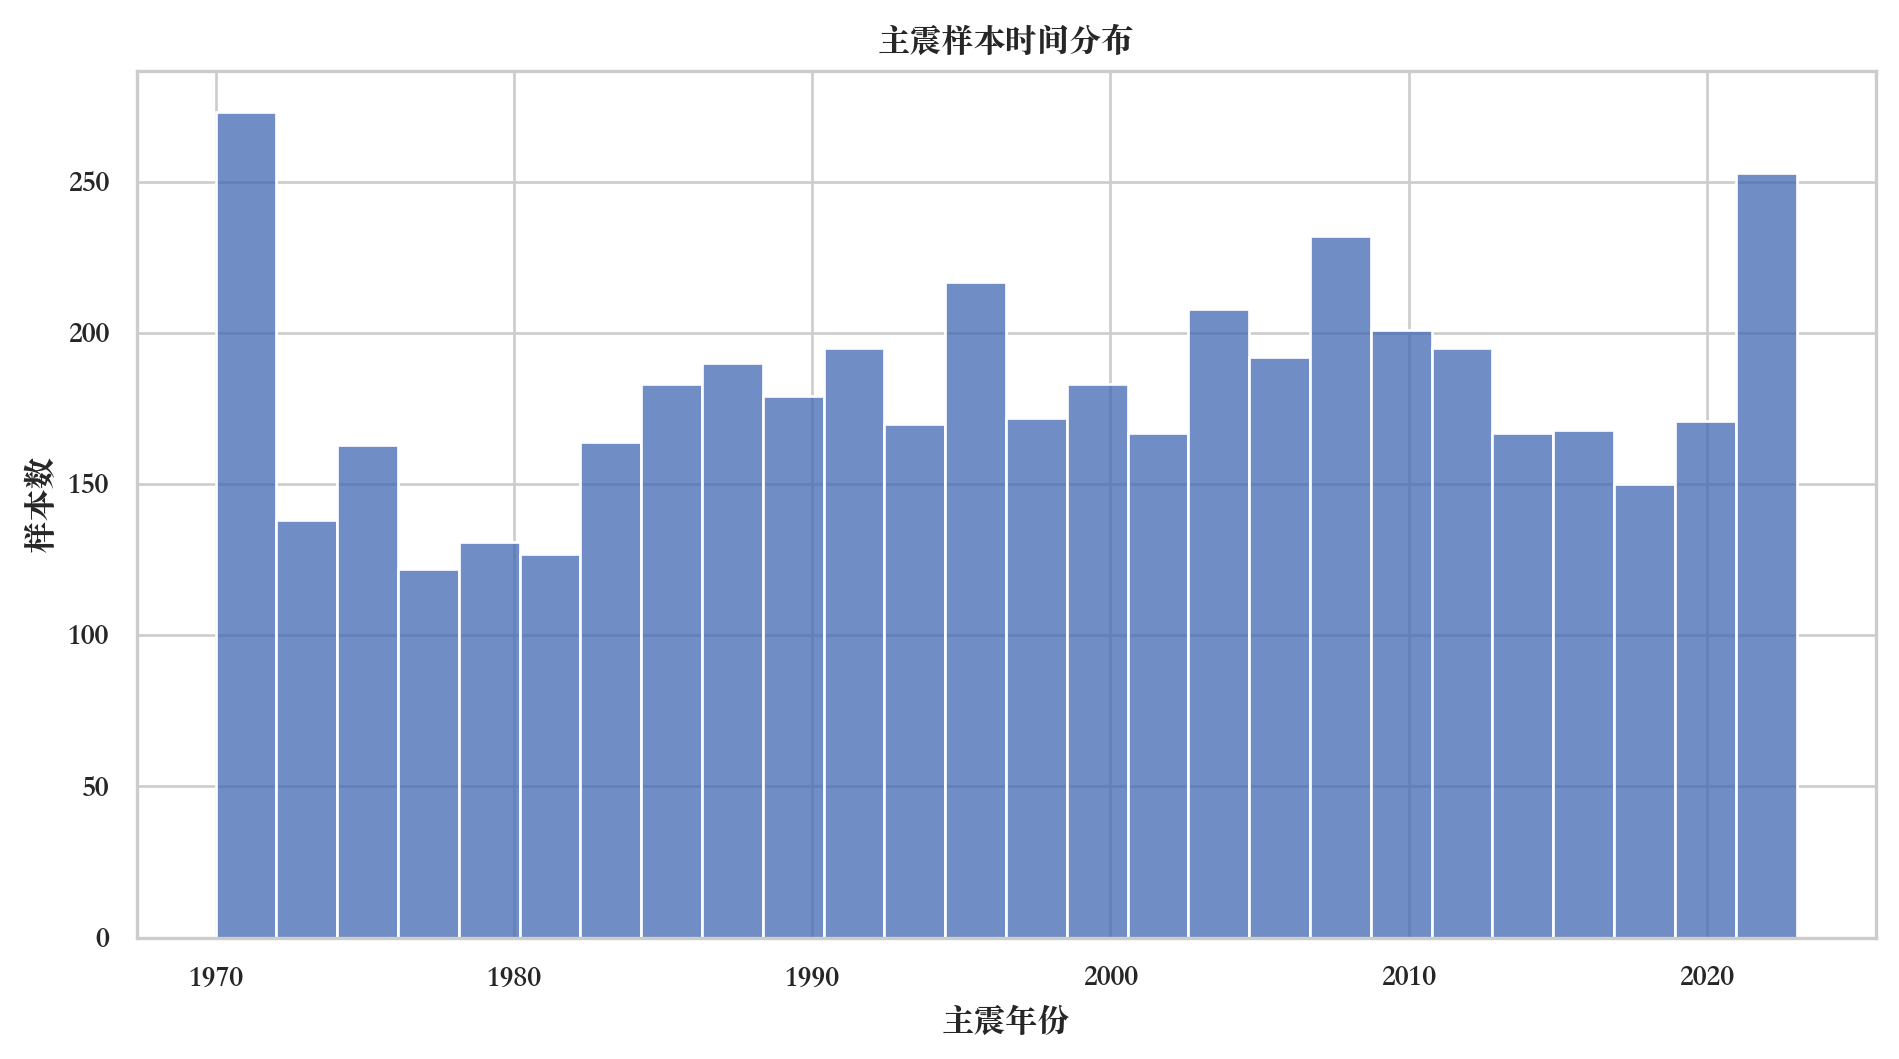
\includegraphics[width=\textwidth]{mainshock_year_distribution.png}
    \caption{主震年份分布}
  \end{subfigure}
  \hfill
  \begin{subfigure}{0.48\textwidth}
    \centering
    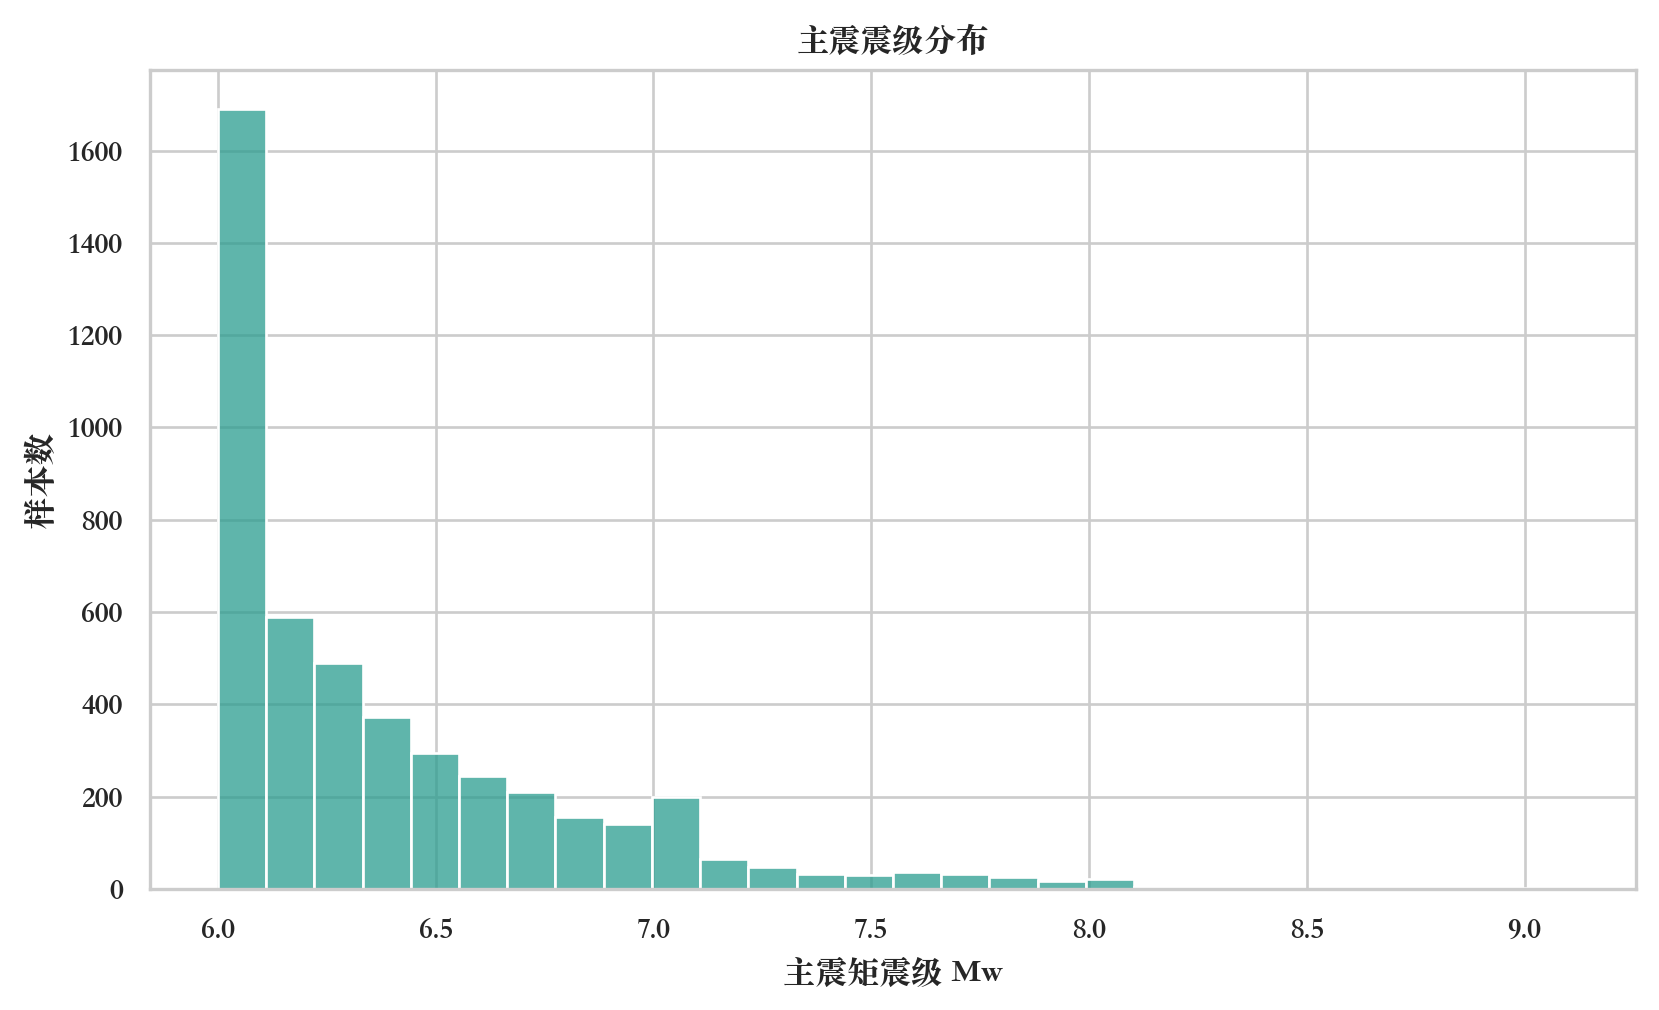
\includegraphics[width=\textwidth]{mainshock_magnitude_distribution.png}
    \caption{主震震级分布}
  \end{subfigure}
  \caption{主震样本分布}
  \label{fig:sample_distribution}
\end{figure}

\section{目标变量分布}
最大余震震级与发生时间分布如图\ref{fig:target_distribution}所示。未来窗口内没有显著余震的样本占比较高，使得 \texttt{target\_max\_mag} 和 \texttt{target\_time\_to\_max\_days} 在 0 附近聚集。与此同时，发生时间目标具有明显长尾，最大值接近 27 天。若直接回归原始时间，模型容易被少数大时间样本主导；因此训练时对时间目标使用
\[
  y_t'=\log(1+y_t)
\]
进行压缩，预测输出再通过 \(\exp(y_t')-1\) 还原到真实天数。

\begin{figure}[H]
  \centering
  \begin{subfigure}{0.48\textwidth}
    \centering
    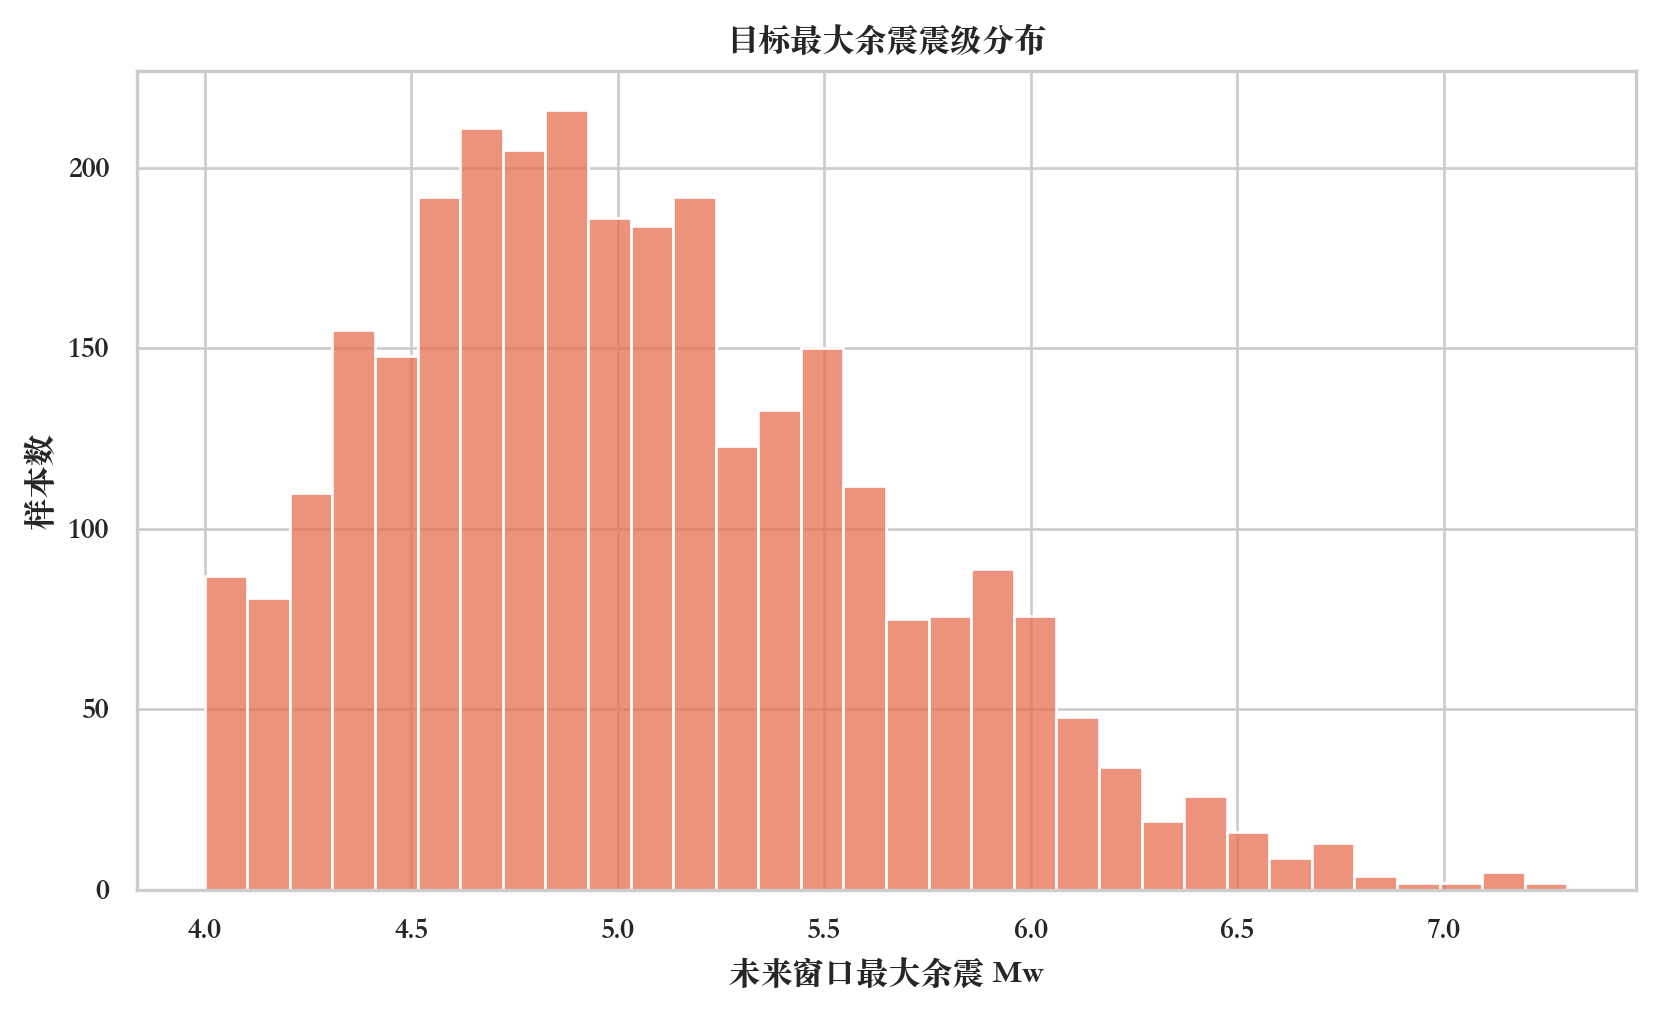
\includegraphics[width=\textwidth]{target_max_mag_distribution.png}
    \caption{目标最大余震震级}
  \end{subfigure}
  \hfill
  \begin{subfigure}{0.48\textwidth}
    \centering
    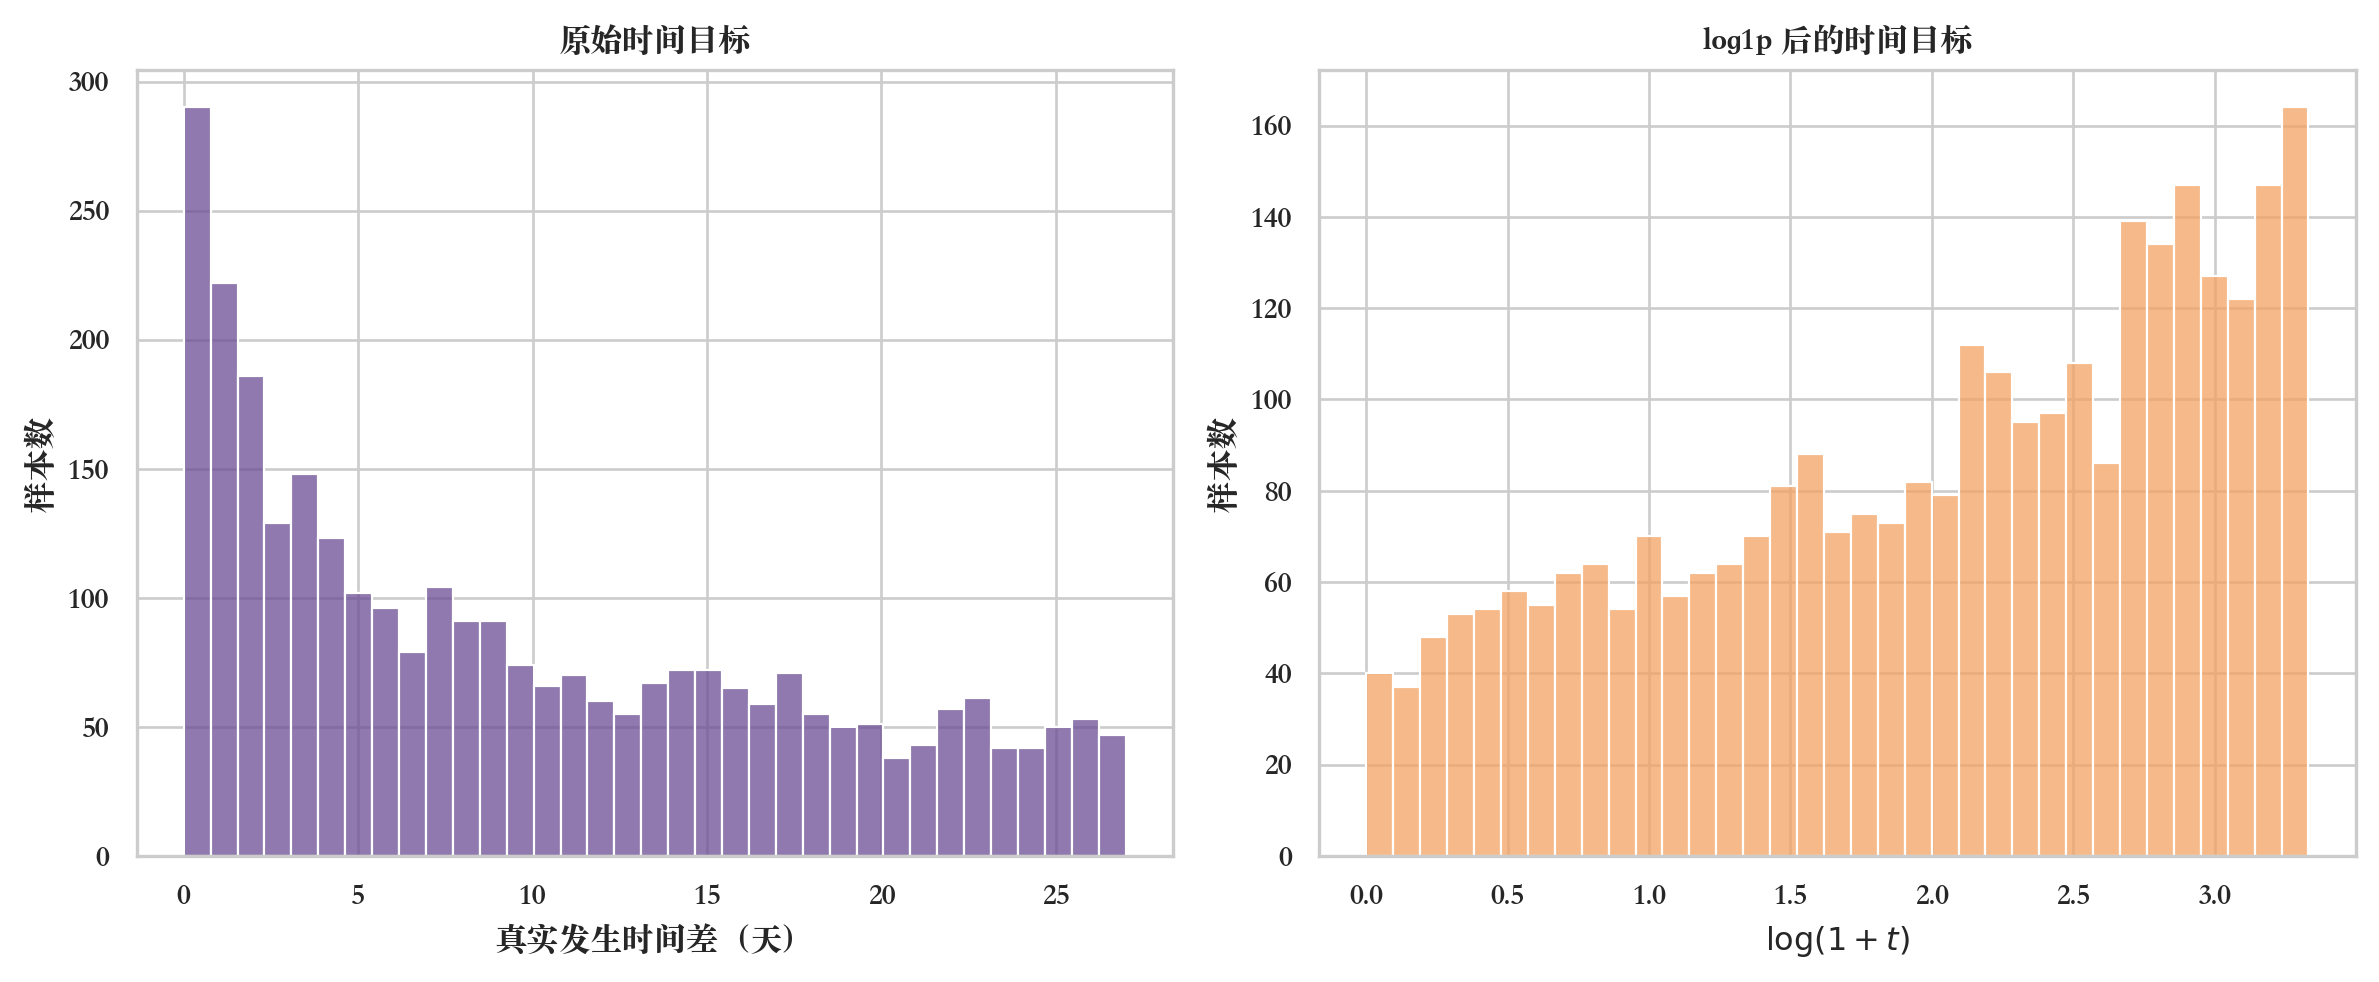
\includegraphics[width=\textwidth]{target_time_log_transform.png}
    \caption{时间目标 log1p 变换}
  \end{subfigure}
  \caption{预测目标分布}
  \label{fig:target_distribution}
\end{figure}

\section{早期余震观测量}
早期余震数量是最直接的序列强度指标。图\ref{fig:early_count}显示，多数主震在 3 天、100 km 窗口内只有少量事件，而少数大震或高余震生产率区域会产生密集余震序列。这种长尾特征使得线性模型难以充分表达，因此树模型和序列模型都更适合捕捉非线性关系。

\begin{figure}[H]
  \centering
  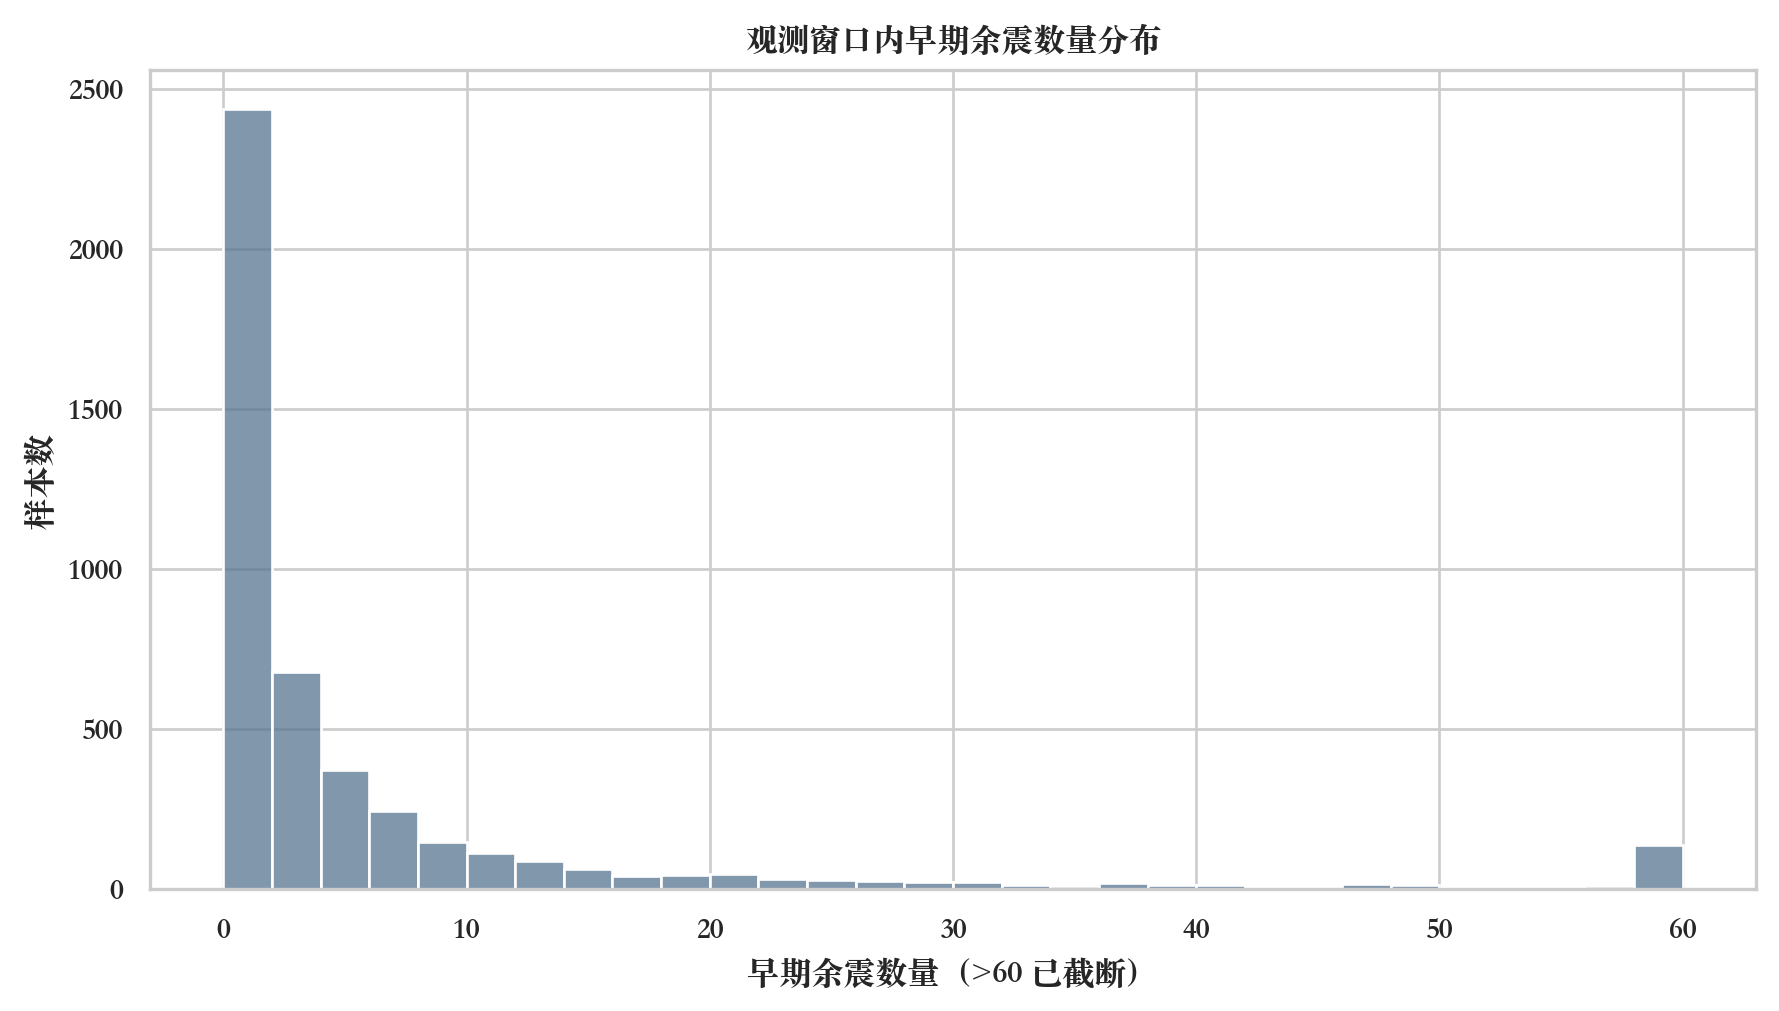
\includegraphics[width=0.72\textwidth]{early_aftershock_count_distribution.png}
  \caption{早期余震数量分布}
  \label{fig:early_count}
\end{figure}

\chapter{高级地震学特征工程}

\section{特征体系总览}
本项目没有只依赖简单统计量，而是将传统地震学规律转化为可学习特征。表\ref{tab:feature_groups}给出了主要特征组及物理含义。

\begin{table}[H]
  \centering
  \caption{核心特征组说明}
  \label{tab:feature_groups}
  \begin{tabular}{p{0.18\textwidth}p{0.28\textwidth}p{0.44\textwidth}}
\toprule
特征组 & 代表字段 & 物理含义 \\
\midrule
地震活动性 & early/count/energy & 早期余震数量、能量、分箱释放过程 \\
G-R 定律 & gr\_b\_value/gr\_a\_value/gr\_mc & MAXC 估计 Mc，Aki-Utsu MLE 估计 b 值 \\
大森-宇津 & omori\_p/omori\_c/omori\_k & 非齐次泊松过程 MLE 拟合余震衰减 \\
Båth/生产率 & bath\_deficit/productivity\_index & 刻画主震后最大余震缺口与生产率水平 \\
空间各向异性 & anisotropy\_* & 用协方差主轴表征破裂方向性 \\
地质构造 & plate\_type\_*/distance & 最近板块边界类型和距离 \\
震源机制 & strike/dip/rake/fault\_type\_* & Global CMT 断层滑动类型与 P/T 轴 \\
\bottomrule
\end{tabular}

\end{table}

\section{Gutenberg--Richter 定律与完整性震级}
Gutenberg--Richter 定律描述某区域内震级不小于 \(M\) 的地震累计频度：
\[
  \log_{10}N(M)=a-bM.
\]
其中 \(b\) 值反映大小地震的相对比例，常被解释为应力状态、介质非均匀性和破裂尺度的统计指示。为了避免将观测不完整的小震纳入估计，本项目采用最大曲率法（Maximum Curvature, MAXC）估计完整性震级 \(M_c\)：对早期余震震级按固定 bin 统计，频次最高的 bin 作为 \(M_c\)。随后使用 Aki--Utsu 极大似然估计：
\[
  b=\frac{\log_{10}e}{\bar{M}-(M_c-\Delta M/2)}.
\]
在得到 \(a\) 与 \(b\) 后，进一步构造地震生产率指数
\[
  I_p=a-bM_{\mathrm{main}},
\]
用于刻画在给定主震震级条件下的相对余震生产能力。

\section{大森--宇津定律与余震衰减}
大森--宇津定律描述余震发生率随时间衰减：
\[
  \lambda(t)=\frac{K}{(t+c)^p}.
\]
其中 \(p\) 控制衰减速度，\(c\) 描述主震后极早期观测不完整或短时饱和效应，\(K\) 近似表征余震生产率。本项目将余震序列视为非齐次泊松过程，最小化负对数似然估计 \(p,c,K\)。若 \(p\) 的优化结果贴近边界，则标记为无效，避免将优化器“撞边界”的结果作为稳定物理参数。

\section{Båth's Law 与早期最大余震缺口}
Båth's Law 经验上认为最大余震通常比主震低约 1.2 级。比赛任务直接预测未来最大余震，因此早期窗口内已经出现的最大余震强度具有重要意义。本项目定义：
\[
  D_{\mathrm{Bath}}=M_{\mathrm{main}}-M_{\mathrm{early,max}}.
\]
若 \(D_{\mathrm{Bath}}\) 较小，说明早期已经出现接近主震规模的较强余震；若缺口较大，则未来仍可能存在显著释放空间。图\ref{fig:bath_productivity}展示了 Båth 缺口和生产率指数与目标最大余震之间的关系。散点较为离散，说明单一物理特征不足以直接决定结果，但其为树模型提供了有效的非线性分裂依据。

\begin{figure}[H]
  \centering
  \begin{subfigure}{0.48\textwidth}
    \centering
    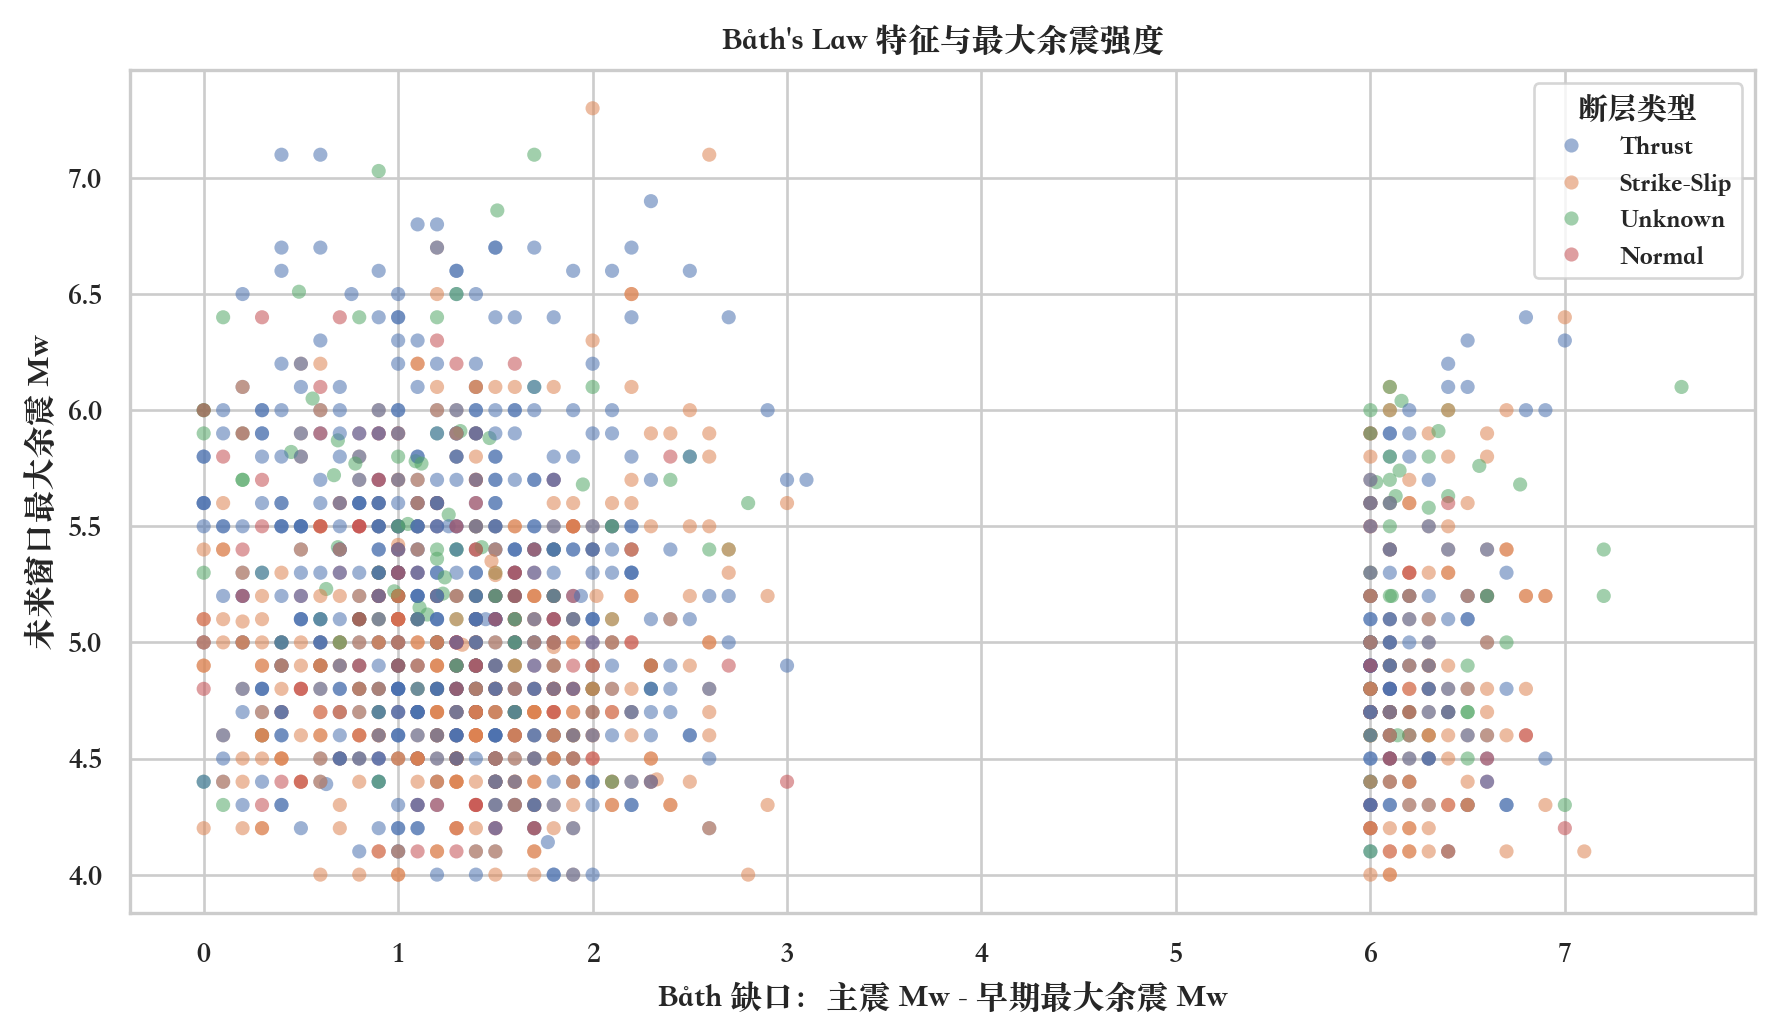
\includegraphics[width=\textwidth]{bath_deficit_vs_target.png}
    \caption{Båth 缺口与最大余震}
  \end{subfigure}
  \hfill
  \begin{subfigure}{0.48\textwidth}
    \centering
    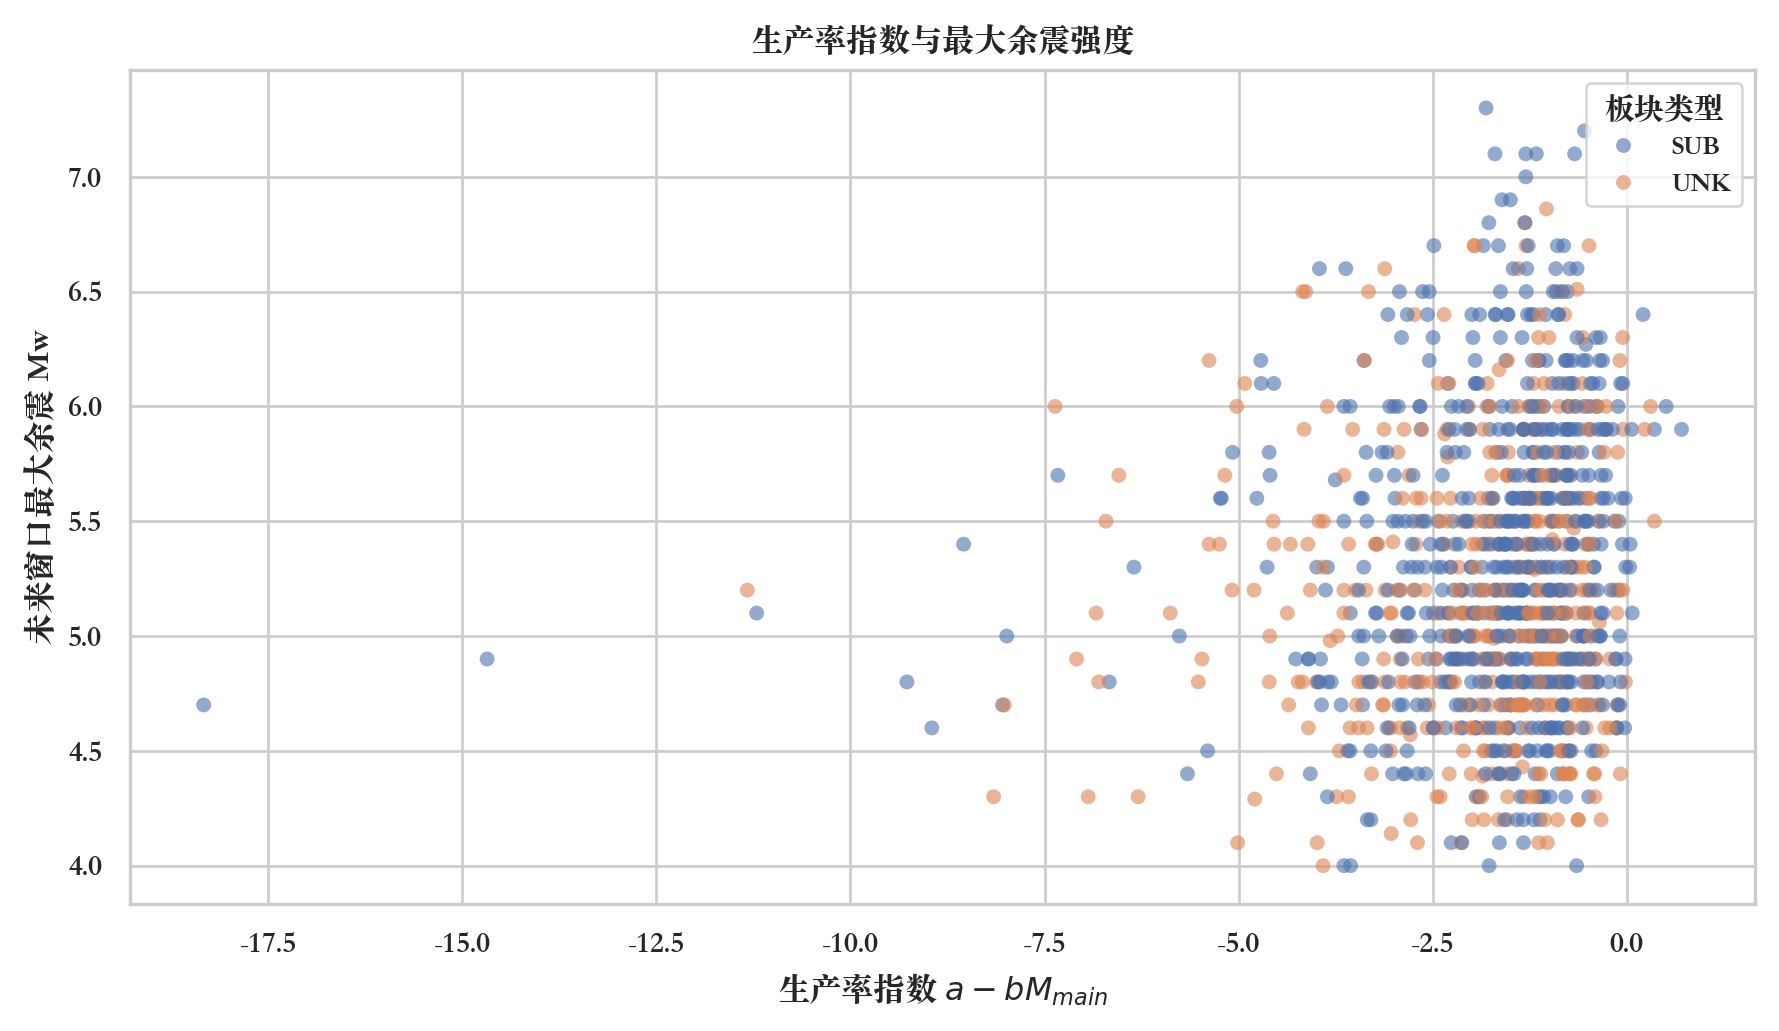
\includegraphics[width=\textwidth]{productivity_index_vs_target.png}
    \caption{生产率指数与最大余震}
  \end{subfigure}
  \caption{地震学先验特征与目标变量关系}
  \label{fig:bath_productivity}
\end{figure}

\section{空间各向异性与断层方向性}
余震往往沿主震破裂面或触发断层带展布。为表征这一方向性，本文将早期余震相对主震位置投影到局部平面：
\[
  x=R_{\oplus}\cos\phi_0(\lambda-\lambda_0), \qquad
  y=R_{\oplus}(\phi-\phi_0).
\]
随后对 \((x,y)\) 坐标计算协方差矩阵并做特征分解，得到主轴长度、短轴长度、长短轴比和方位角。若早期余震数少于 3 条，则各向异性特征标记为无效。

\section{构造背景与震源机制}
板块边界距离与边界类型反映主震所处构造背景。PB2002 边界数据被读取为 GeoDataFrame 后，通过最近邻空间连接获得主震到最近板块边界的近似距离和类别。当前样本中最近边界类型以 SUB 和 UNK 为主，分布如图\ref{fig:geology_distribution}所示。

Global CMT 震源机制进一步提供断层滑动方向。本文采用严格匹配条件：主震时间差小于 60 秒，空间距离小于 50 km。有效匹配样本为 4022 条，最大时间差 11.84 秒，最大距离 46.75 km。根据 \(rake_1\) 将断层类型划分为 Thrust、Normal、Strike-Slip 与 Unknown。图\ref{fig:geology_distribution}同时展示了震源机制类型分布，走滑型和逆冲型样本占比较高。

\begin{figure}[H]
  \centering
  \begin{subfigure}{0.32\textwidth}
    \centering
    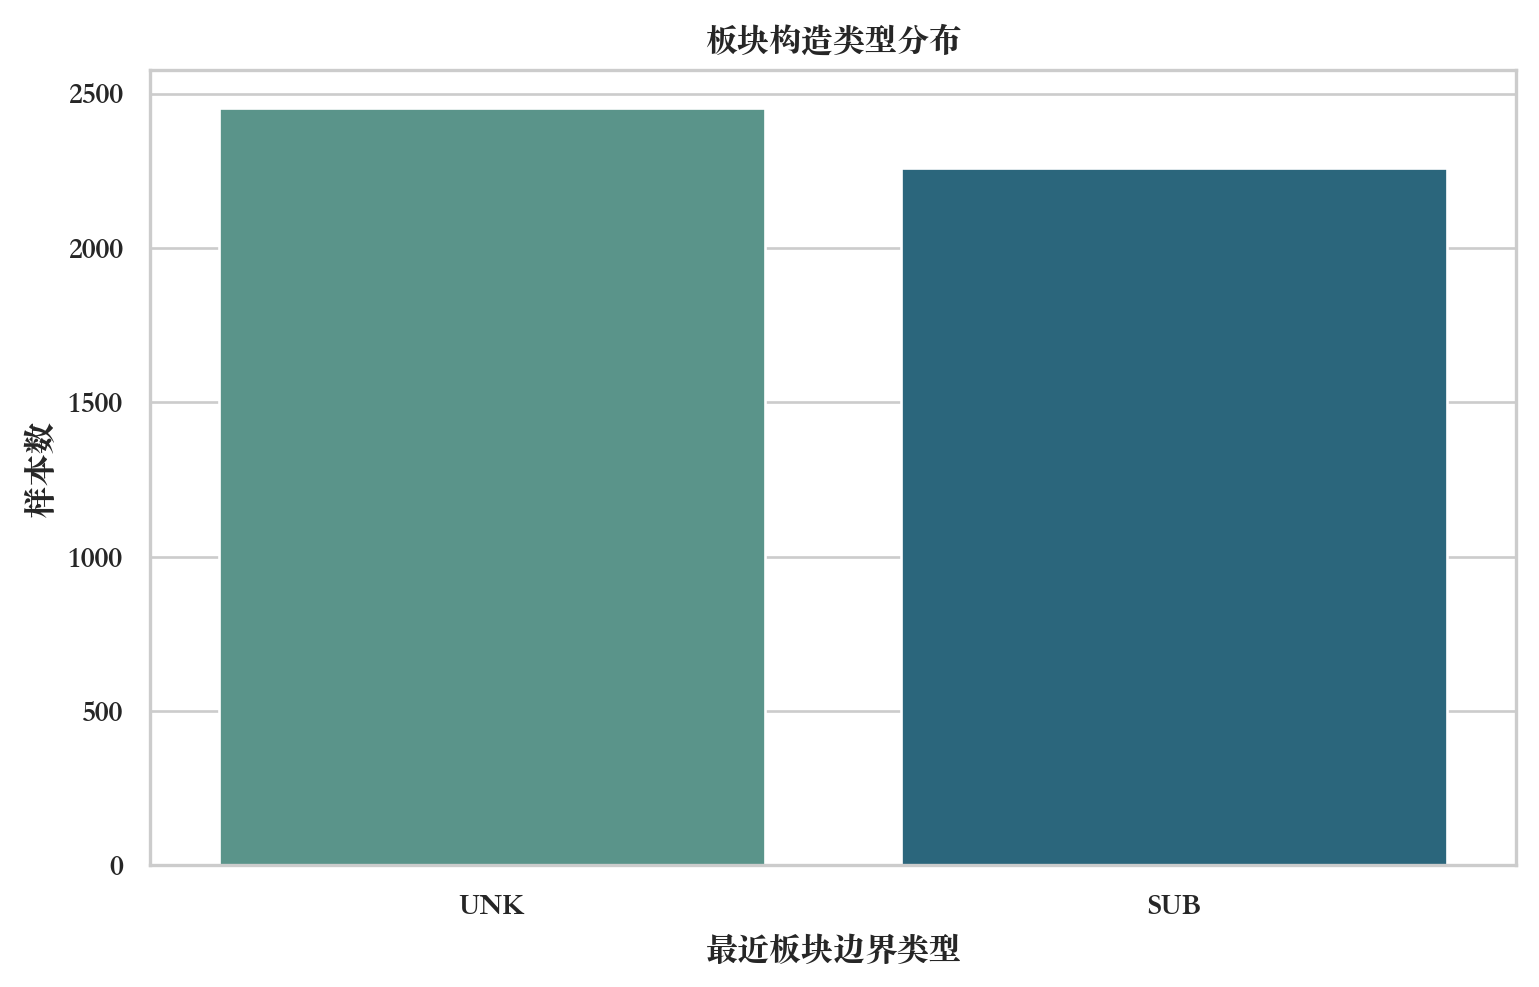
\includegraphics[width=\textwidth]{plate_type_distribution.png}
    \caption{板块边界类型}
  \end{subfigure}
  \hfill
  \begin{subfigure}{0.32\textwidth}
    \centering
    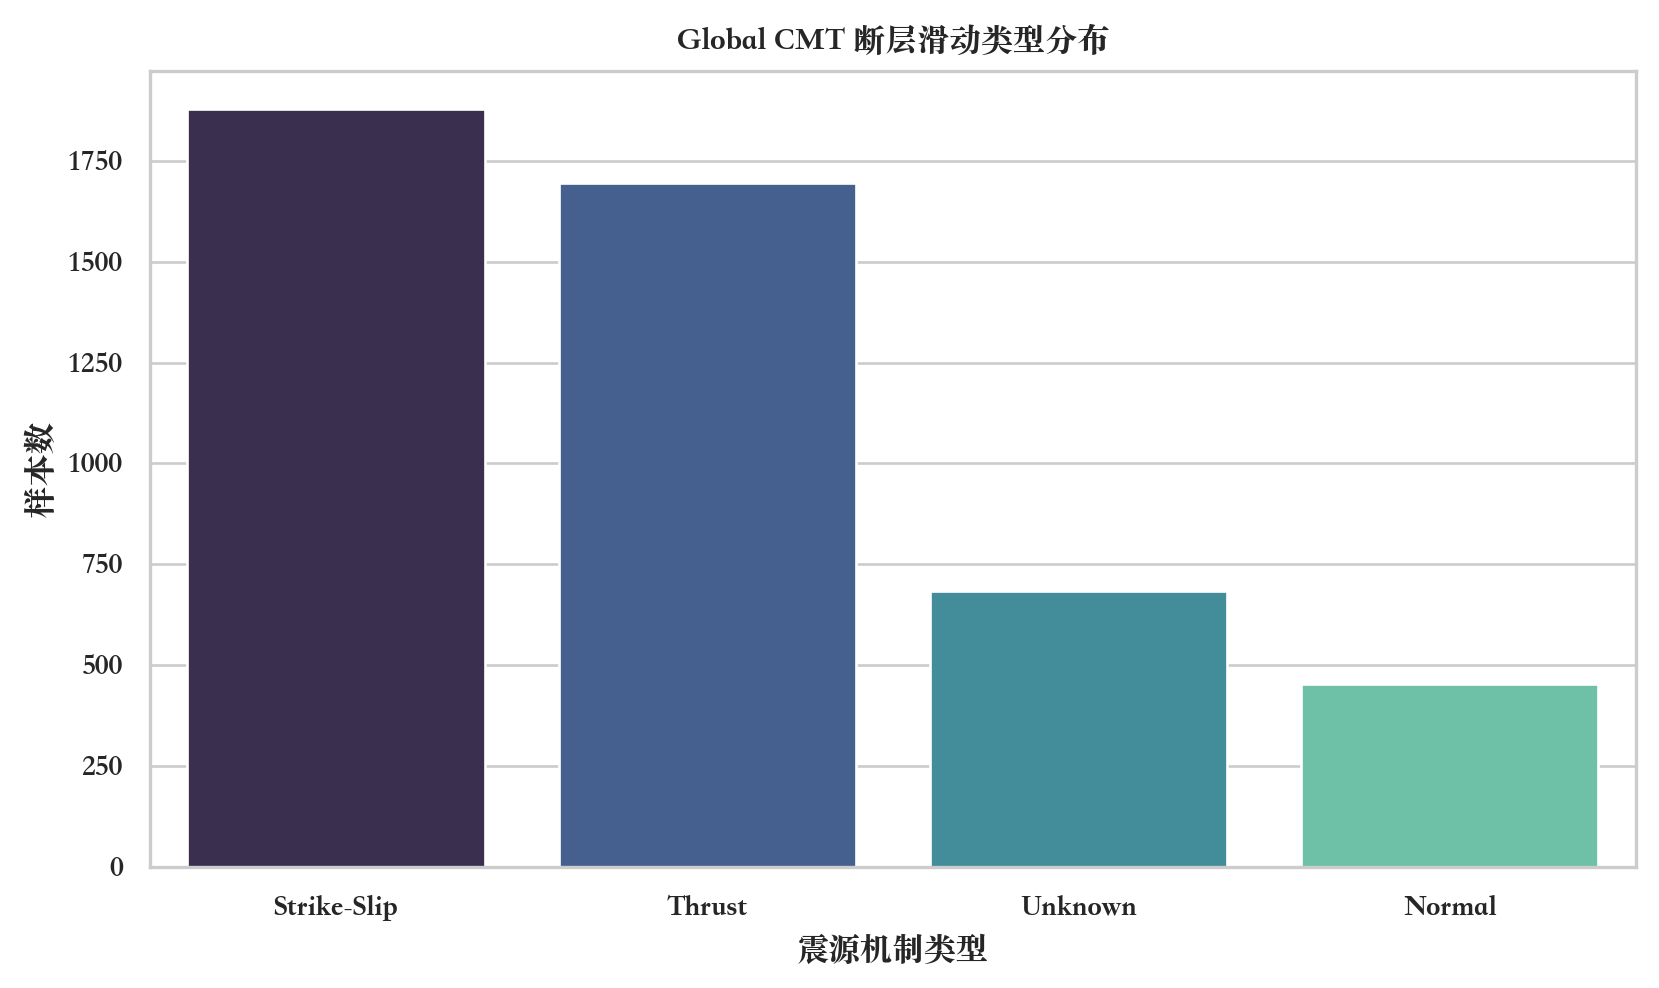
\includegraphics[width=\textwidth]{fault_type_distribution.png}
    \caption{断层滑动类型}
  \end{subfigure}
  \hfill
  \begin{subfigure}{0.32\textwidth}
    \centering
    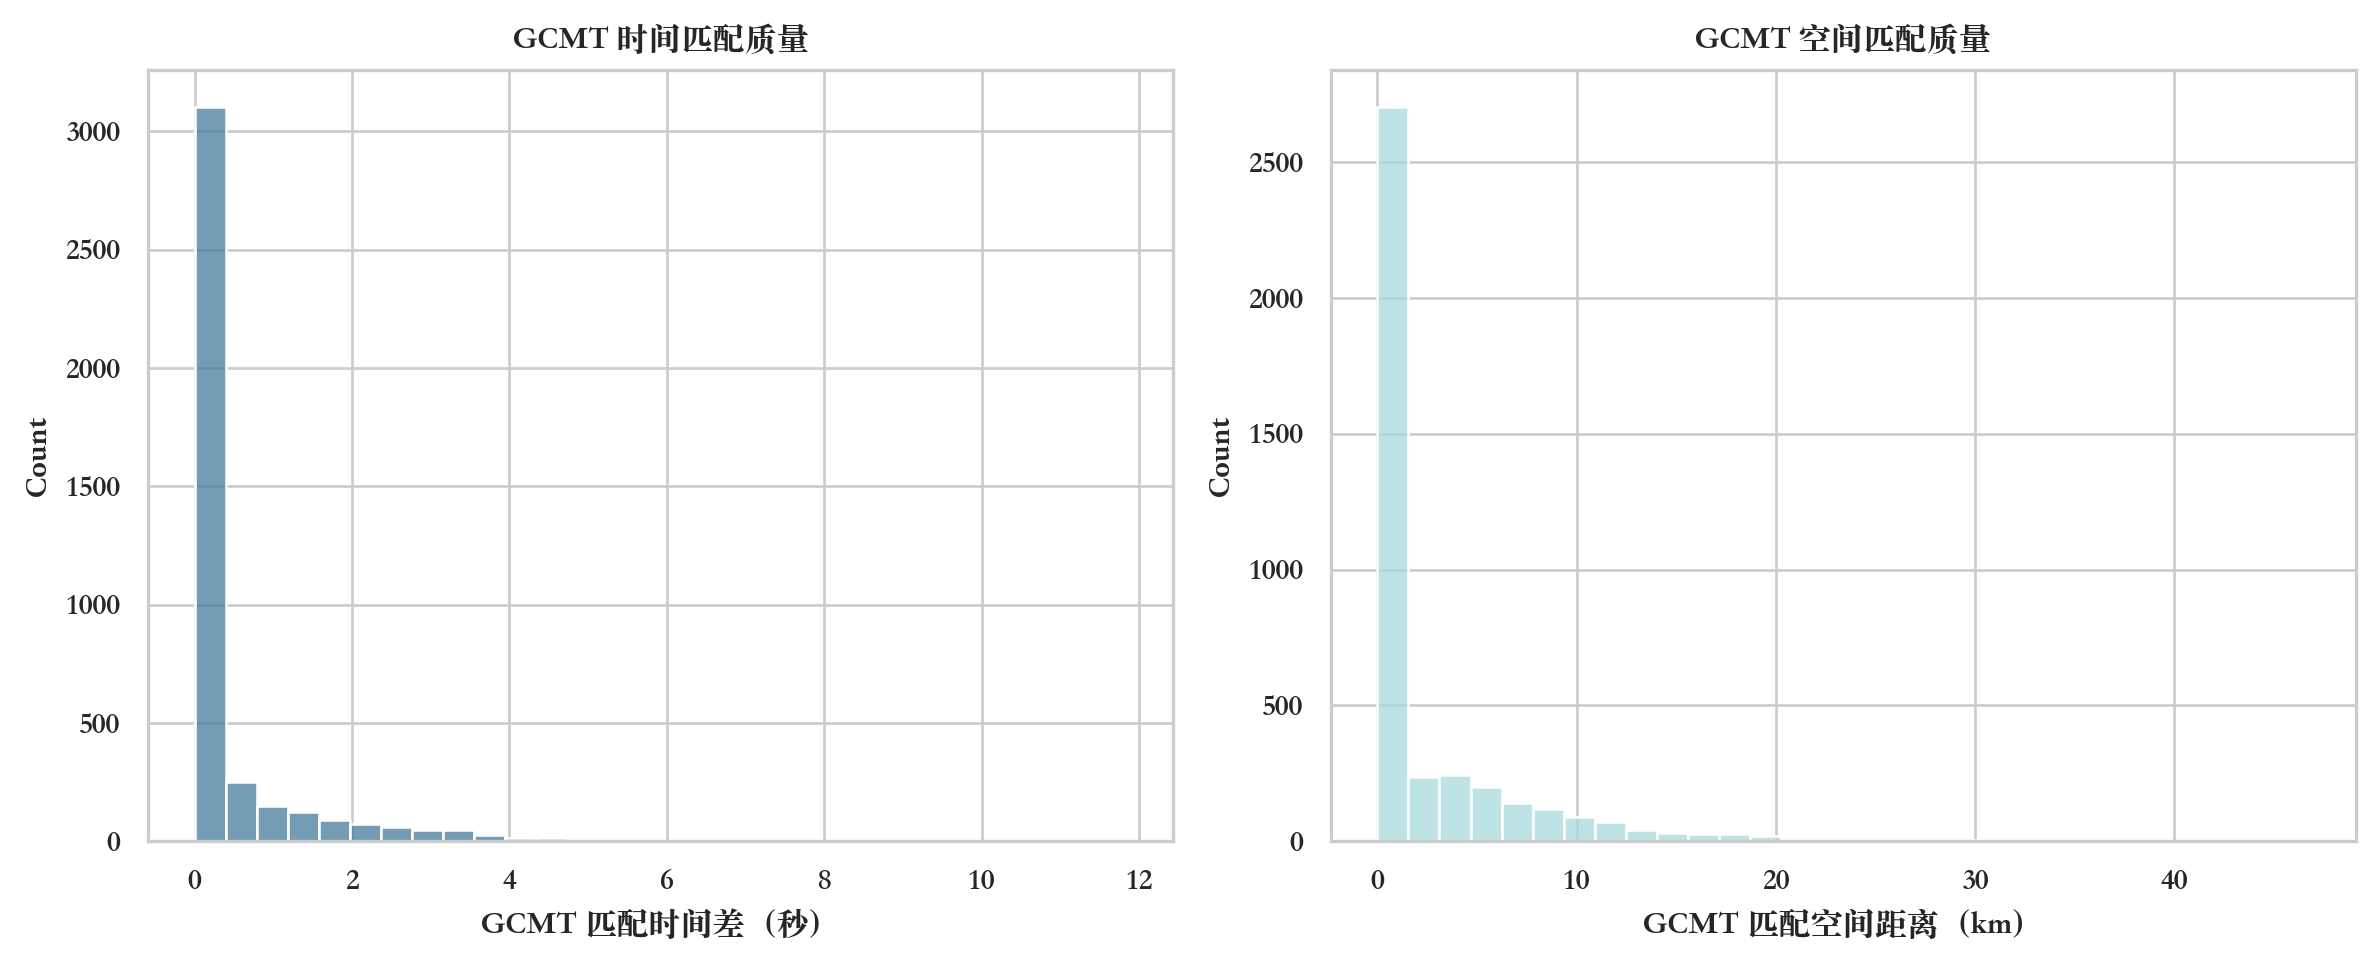
\includegraphics[width=\textwidth]{gcmt_match_quality.png}
    \caption{GCMT 匹配质量}
  \end{subfigure}
  \caption{构造背景与震源机制特征}
  \label{fig:geology_distribution}
\end{figure}

\section{特征有效性分析}
由于部分物理模型要求最小事件数，所有高级特征并非对每个样本都有效。表\ref{tab:feature_validity}和图\ref{fig:feature_validity}给出了特征有效率。GCMT 震源机制有效率最高，达到 85.50\%；Båth 特征有效率为 63.80\%；G-R b 值有效率约为 25.87\%；Omori 和 ETAS 对事件数要求更高，有效率较低。这一结果提示后续若要提高物理参数覆盖率，需要更完整的低震级局部目录。

\begin{table}[H]
  \centering
  \caption{高级特征有效率统计}
  \label{tab:feature_validity}
  \begingroup
\footnotesize
\setlength{\tabcolsep}{4pt}
\begin{tabular}{lrr}
\toprule
特征模块 & 有效样本数 & 有效率 \\
\midrule
G-R b 值 & 1218 & 25.85\% \\
Omori 参数 & 503 & 10.68\% \\
空间各向异性 & 1854 & 39.35\% \\
ETAS 参数 & 800 & 16.98\% \\
Båth 特征 & 3004 & 63.77\% \\
GCMT 震源机制 & 4028 & 85.50\% \\
\bottomrule
\end{tabular}
\endgroup

\end{table}

\begin{figure}[H]
  \centering
  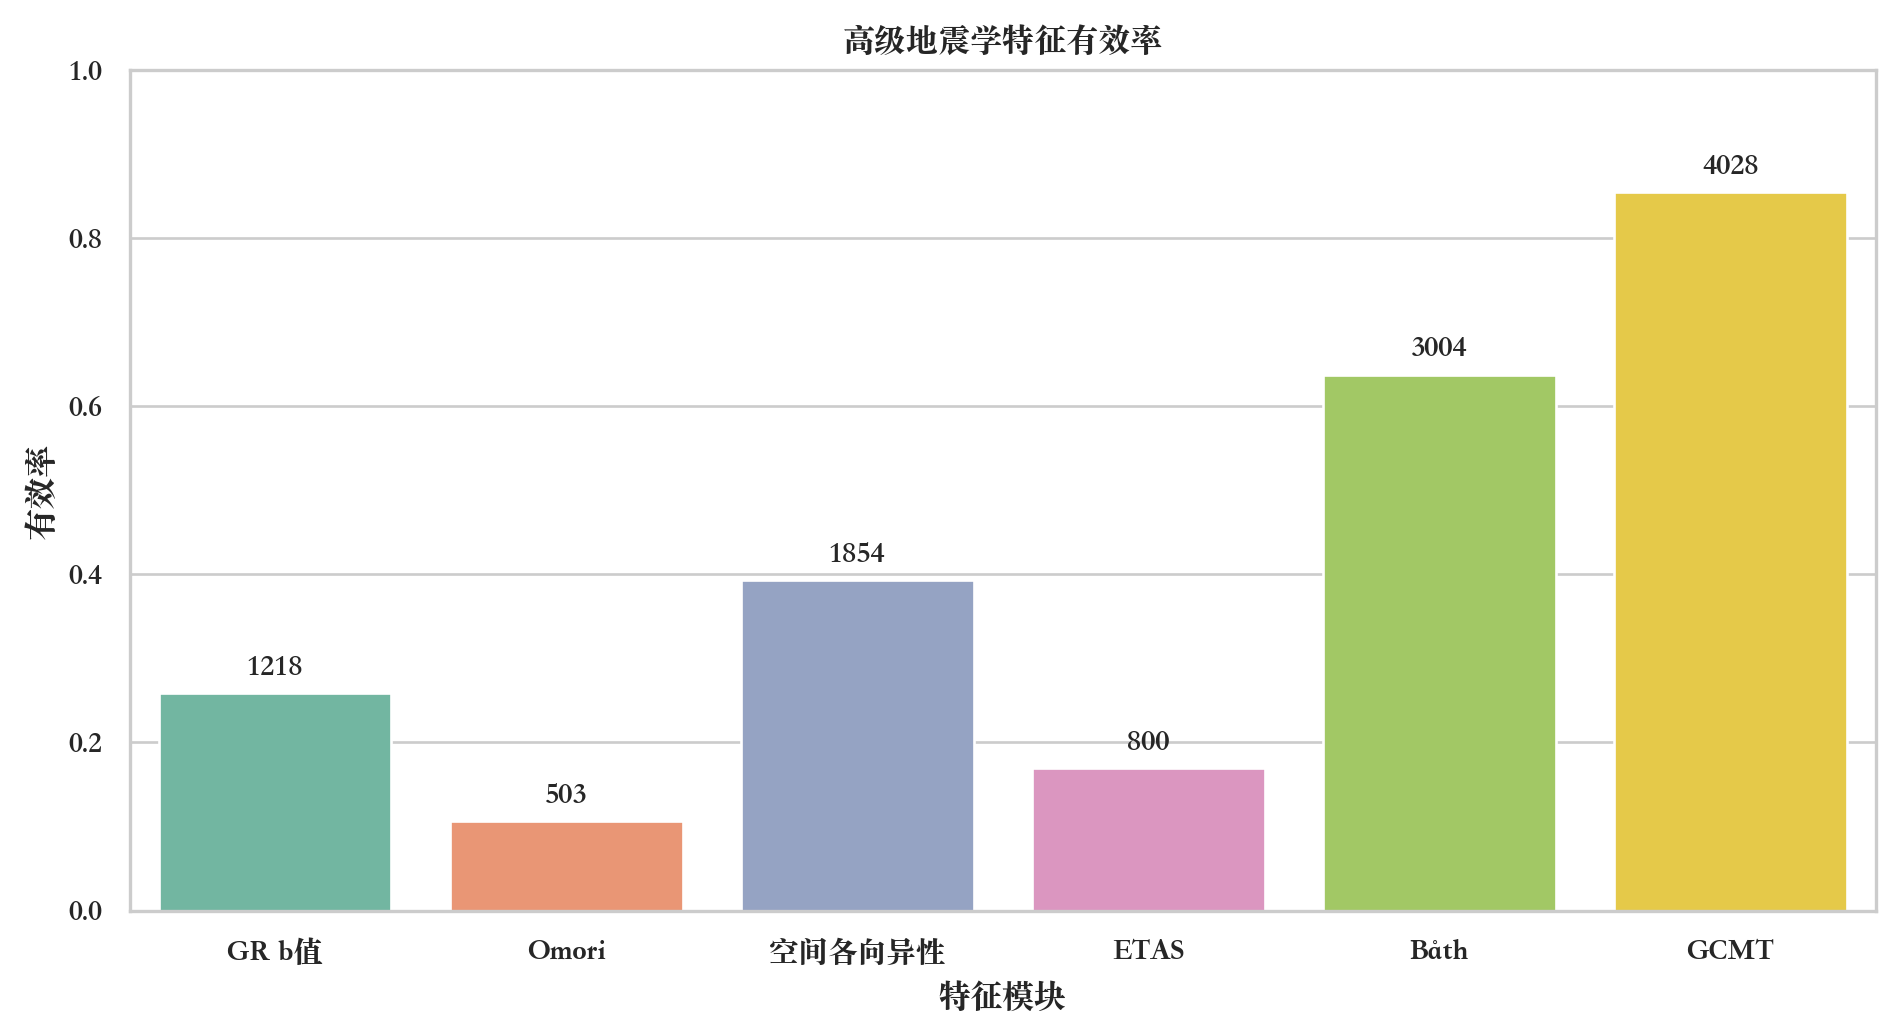
\includegraphics[width=0.78\textwidth]{feature_validity_bar.png}
  \caption{高级特征有效率柱状图}
  \label{fig:feature_validity}
\end{figure}

\chapter{模型方法}

\section{机器学习基线}
树模型是当前工程的稳定主线。LightGBM 与 XGBoost 都能处理非线性特征交互，并对缺失值具有较好鲁棒性，适合当前“物理特征部分缺失、类别 one-hot 与连续变量混合”的特征结构。项目中训练两个目标：最大余震震级与最大余震时间。震级目标保持原尺度，时间目标使用 \(\log(1+t)\) 长尾压缩。

LightGBM 的时间目标额外支持非对称自定义损失。设真实时间为 \(t\)，预测时间为 \(\hat{t}\)，若 \(\hat{t}>t\)，表示预测晚于实际发生时间，预警场景下风险更高。因此定义：
\[
  \loss_t =
  \begin{cases}
    \alpha(\hat{t}-t)^2, & \hat{t}>t,\\
    (\hat{t}-t)^2, & \hat{t}\le t,
  \end{cases}
  \quad \alpha=2.
\]
该损失在真实天数尺度判断“偏晚”，并通过链式法则返回 log 预测尺度上的梯度和 Hessian，使训练目标与业务风险更一致。

\section{Transformer 双输入融合模型}
深度学习模型采用“事件序列 + 全局特征”的双输入结构。早期余震序列被编码为
\[
  x_i=[\Delta t_i,\log(1+\Delta t_i),\Delta x_i,\Delta y_i,d_i,\mathrm{depth}_i,M_i],
\]
经线性投影和正弦位置编码送入 Transformer Encoder。全局手工特征经 MLP 编码后与序列池化向量拼接，最终输出震级和 log 时间。为避免数据泄漏，序列特征与全局特征的 RobustScaler 只在时间切分后的训练集上拟合，验证和推理阶段只复用已保存预处理器。

\section{ST-GNN 有向时空因果图}
仅用 Transformer 处理序列会弱化余震空间传播结构。ST-GNN 将每个早期余震事件视为图节点，并构建有向时空边。给定事件 \(i,j\)，仅当
\[
  d_{ij}<R_g,\qquad t_i<t_j
\]
时，才允许边 \(i\rightarrow j\) 存在。消息传递采用 \(A[\mathrm{target},\mathrm{source}]\) 约定，即未来节点只能聚合过去节点的信息，避免信息从未来倒流。边权使用高斯核：
\[
  A_{ji}=\exp\left(-\frac{d_{ij}^{2}}{2\sigma^{2}}\right).
\]
图\ref{fig:stgnn}展示了该有向因果构图方式。该模型目前作为可选增强路径，默认一键流程仍采用树模型提交，以保证速度和稳定性。

\begin{figure}[H]
  \centering
  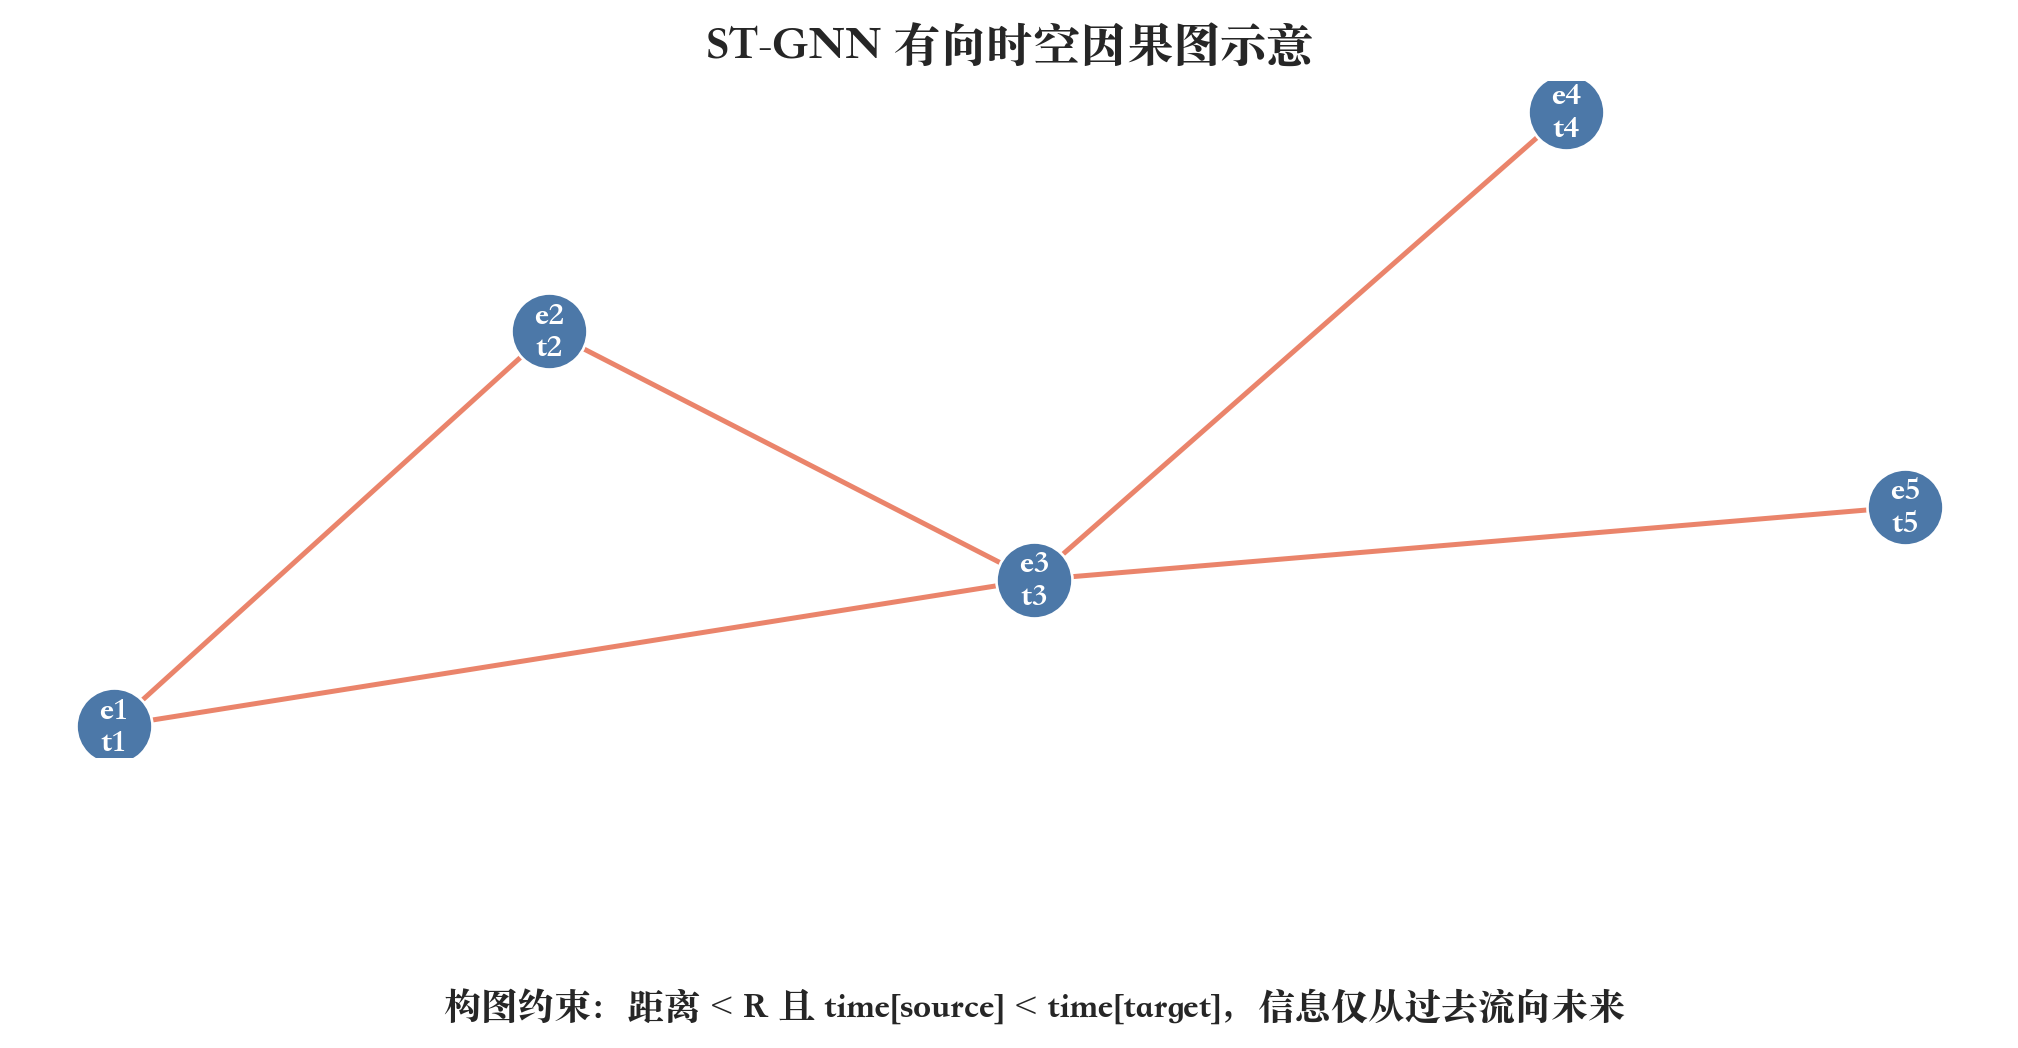
\includegraphics[width=0.80\textwidth]{stgnn_causal_graph.png}
  \caption{ST-GNN 有向时空因果图示意}
  \label{fig:stgnn}
\end{figure}

\chapter{评估体系与防泄漏设计}

\section{时间序列交叉验证}
地震目录具有强时间顺序属性。若随机 K 折划分，模型可能在训练阶段看到未来年份的构造分布和地震序列特征，从而造成数据穿越。本项目使用 TimeSeriesSplit：每一折都使用更早时间段训练，验证集严格位于训练集之后。表\ref{tab:cv_fold_metrics}列出了每折训练后的验证时间段与指标。

\begin{center}
\begingroup
\footnotesize
\setlength{\tabcolsep}{4pt}
\begin{longtable}{clllrrr}
\toprule
Fold & 模型 & 验证起点 & 验证终点 & Mag RMSE & Time RMSE & Asym MAE \\
\midrule
\endfirsthead
\toprule
Fold & 模型 & 验证起点 & 验证终点 & Mag RMSE & Time RMSE & Asym MAE \\
\midrule
\endhead
1 & baseline & 1984-07-02 & 1993-12-09 & 0.543 & 8.448 & 9.403 \\
1 & xgboost & 1984-07-02 & 1993-12-09 & 0.539 & 8.704 & 8.579 \\
2 & baseline & 1993-12-10 & 2002-01-28 & 0.580 & 8.446 & 9.147 \\
2 & xgboost & 1993-12-10 & 2002-01-28 & 0.571 & 8.654 & 8.400 \\
3 & baseline & 2002-02-03 & 2008-11-22 & 0.540 & 8.601 & 9.485 \\
3 & xgboost & 2002-02-03 & 2008-11-22 & 0.533 & 8.621 & 8.775 \\
4 & baseline & 2008-11-22 & 2016-02-17 & 0.511 & 8.082 & 9.037 \\
4 & xgboost & 2008-11-22 & 2016-02-17 & 0.505 & 8.465 & 8.448 \\
5 & baseline & 2016-03-02 & 2023-12-21 & 0.480 & 8.193 & 9.104 \\
5 & xgboost & 2016-03-02 & 2023-12-21 & 0.473 & 8.414 & 8.371 \\
\bottomrule
\end{longtable}
\endgroup

\captionof{table}{时间序列交叉验证每折指标}
\label{tab:cv_fold_metrics}
\end{center}

\section{评估指标}
常规指标包括震级 RMSE/MAE 与时间 RMSE/MAE：
\[
  \mathrm{RMSE}=\sqrt{\frac{1}{n}\sum_{i=1}^{n}(\hat{y}_i-y_i)^2},\qquad
  \mathrm{MAE}=\frac{1}{n}\sum_{i=1}^{n}|\hat{y}_i-y_i|.
\]
考虑预警场景下“预测偏晚”的风险更大，本文还计算非对称时间误差：
\[
  \mathrm{AsymMAE}=\frac{1}{n}\sum_i w_i |\hat{t}_i-t_i|,
  \quad
  w_i=
  \begin{cases}
    2, & \hat{t}_i>t_i,\\
    1, & \hat{t}_i\le t_i.
  \end{cases}
\]
该指标将模型从纯数值拟合引向预警风险控制。

\section{深度学习预处理防泄漏}
深度模型对尺度敏感，但 scaler 的拟合如果在全量数据上完成，会将未来验证集分布泄漏给训练过程。因此项目采用如下策略：
\begin{enumerate}[label=\arabic*.]
  \item 先按 \texttt{mainshock\_time} 排序并切分训练集、验证集；
  \item 仅用训练集调用 \texttt{fit\_dataset\_preprocessors}；
  \item Dataset 构造阶段只接收并 transform，不在内部 fit；
  \item 预处理器随模型一同保存，推理时复用同一对象。
\end{enumerate}
这一设计保证深度模型与树模型遵循同样的时间因果原则。

\chapter{实验结果与分析}

\section{交叉验证结果}
平均验证指标见表\ref{tab:model_mean_metrics}。LightGBM 与 XGBoost 的震级 RMSE 非常接近，XGBoost 在时间 MAE 与非对称 MAE 上更优，因此最终 OOF 融合给予 XGBoost 更高权重。图\ref{fig:cv_metrics}进一步展示了各折 RMSE 与时间非对称指标变化。第三折时间 RMSE 较高，说明 1998--2006 年段可能包含更复杂或更极端的余震序列，对模型泛化提出挑战。

\begin{table}[H]
  \centering
  \caption{模型平均验证指标}
  \label{tab:model_mean_metrics}
  \begingroup
\footnotesize
\setlength{\tabcolsep}{4pt}
\begin{tabular}{p{0.16\textwidth}rrrrrr}
\toprule
模型 & Mag RMSE & Mag MAE & Time RMSE & Time MAE & Asym MAE & Asym RMSE \\
\midrule
baseline & 0.531 & 0.425 & 8.354 & 6.729 & 9.235 & 9.374 \\
xgboost & 0.524 & 0.421 & 8.572 & 6.716 & 8.515 & 9.167 \\
\bottomrule
\end{tabular}
\endgroup

\end{table}

\begin{figure}[H]
  \centering
  \begin{subfigure}{0.48\textwidth}
    \centering
    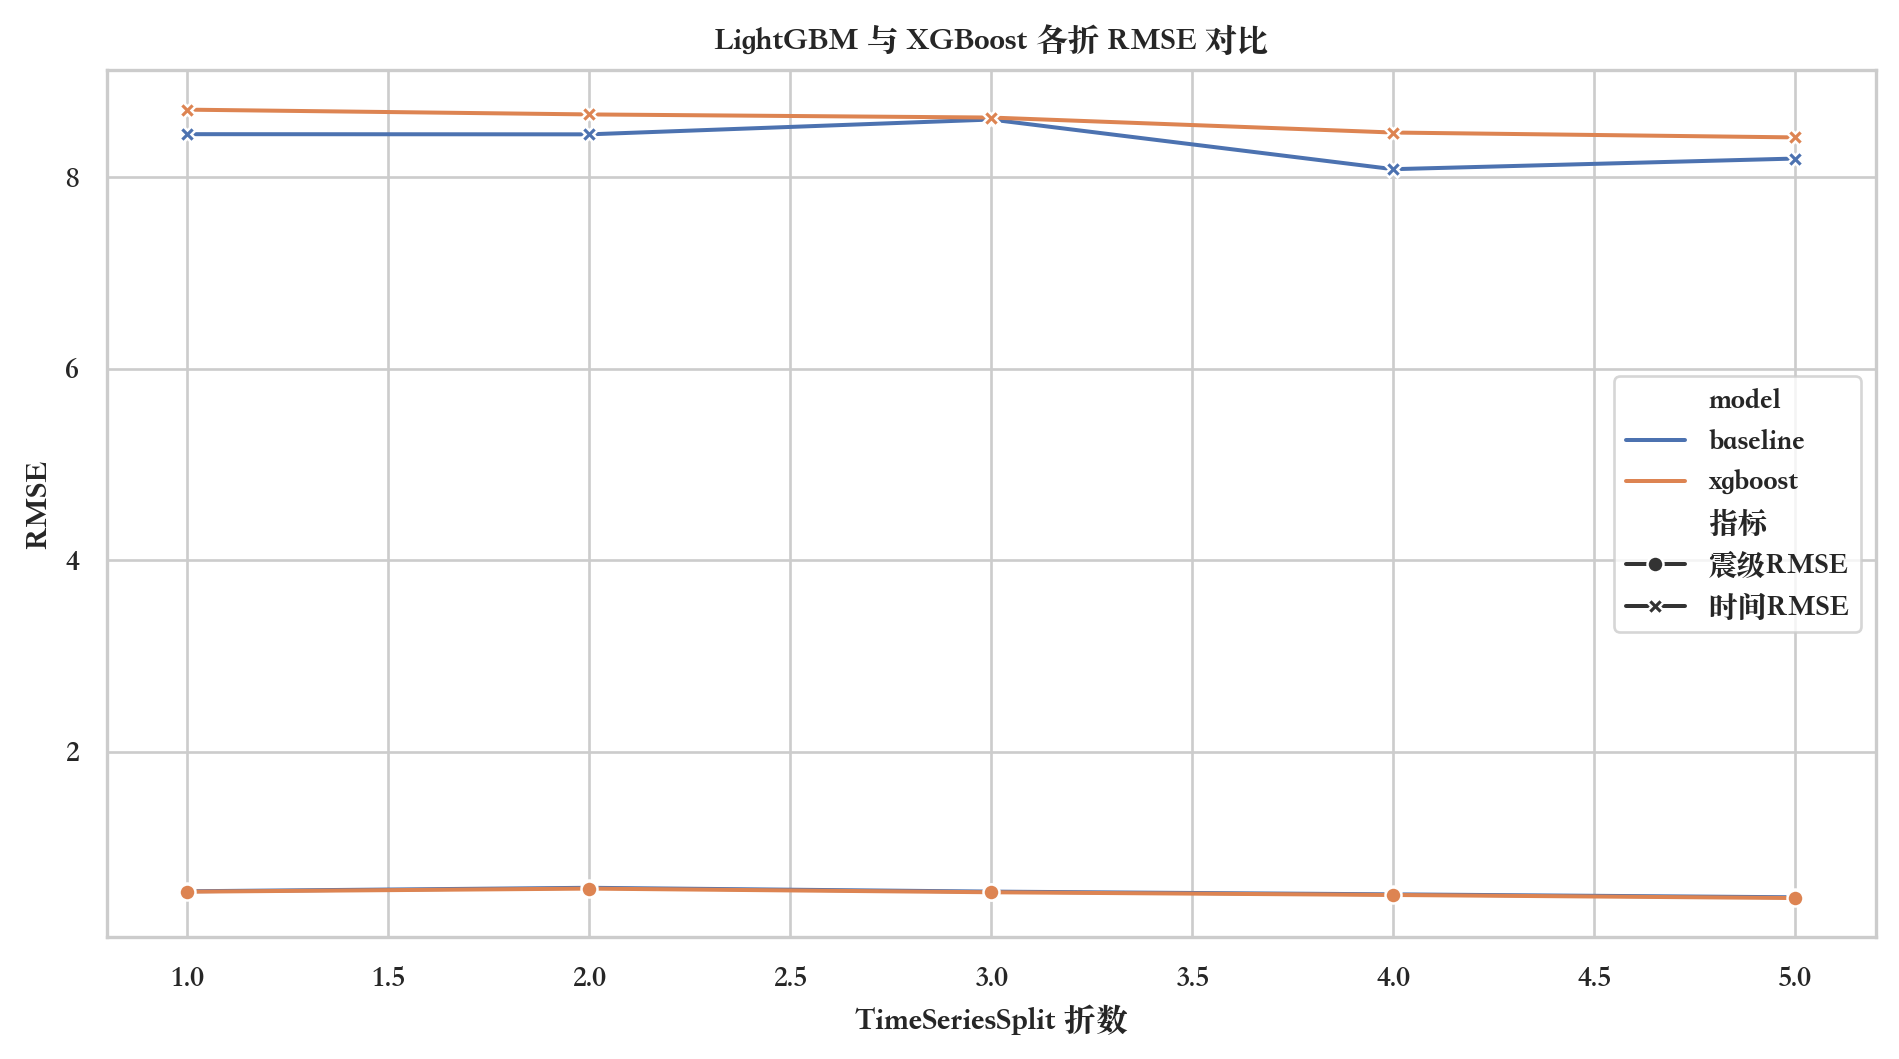
\includegraphics[width=\textwidth]{cv_rmse_by_fold.png}
    \caption{各折 RMSE}
  \end{subfigure}
  \hfill
  \begin{subfigure}{0.48\textwidth}
    \centering
    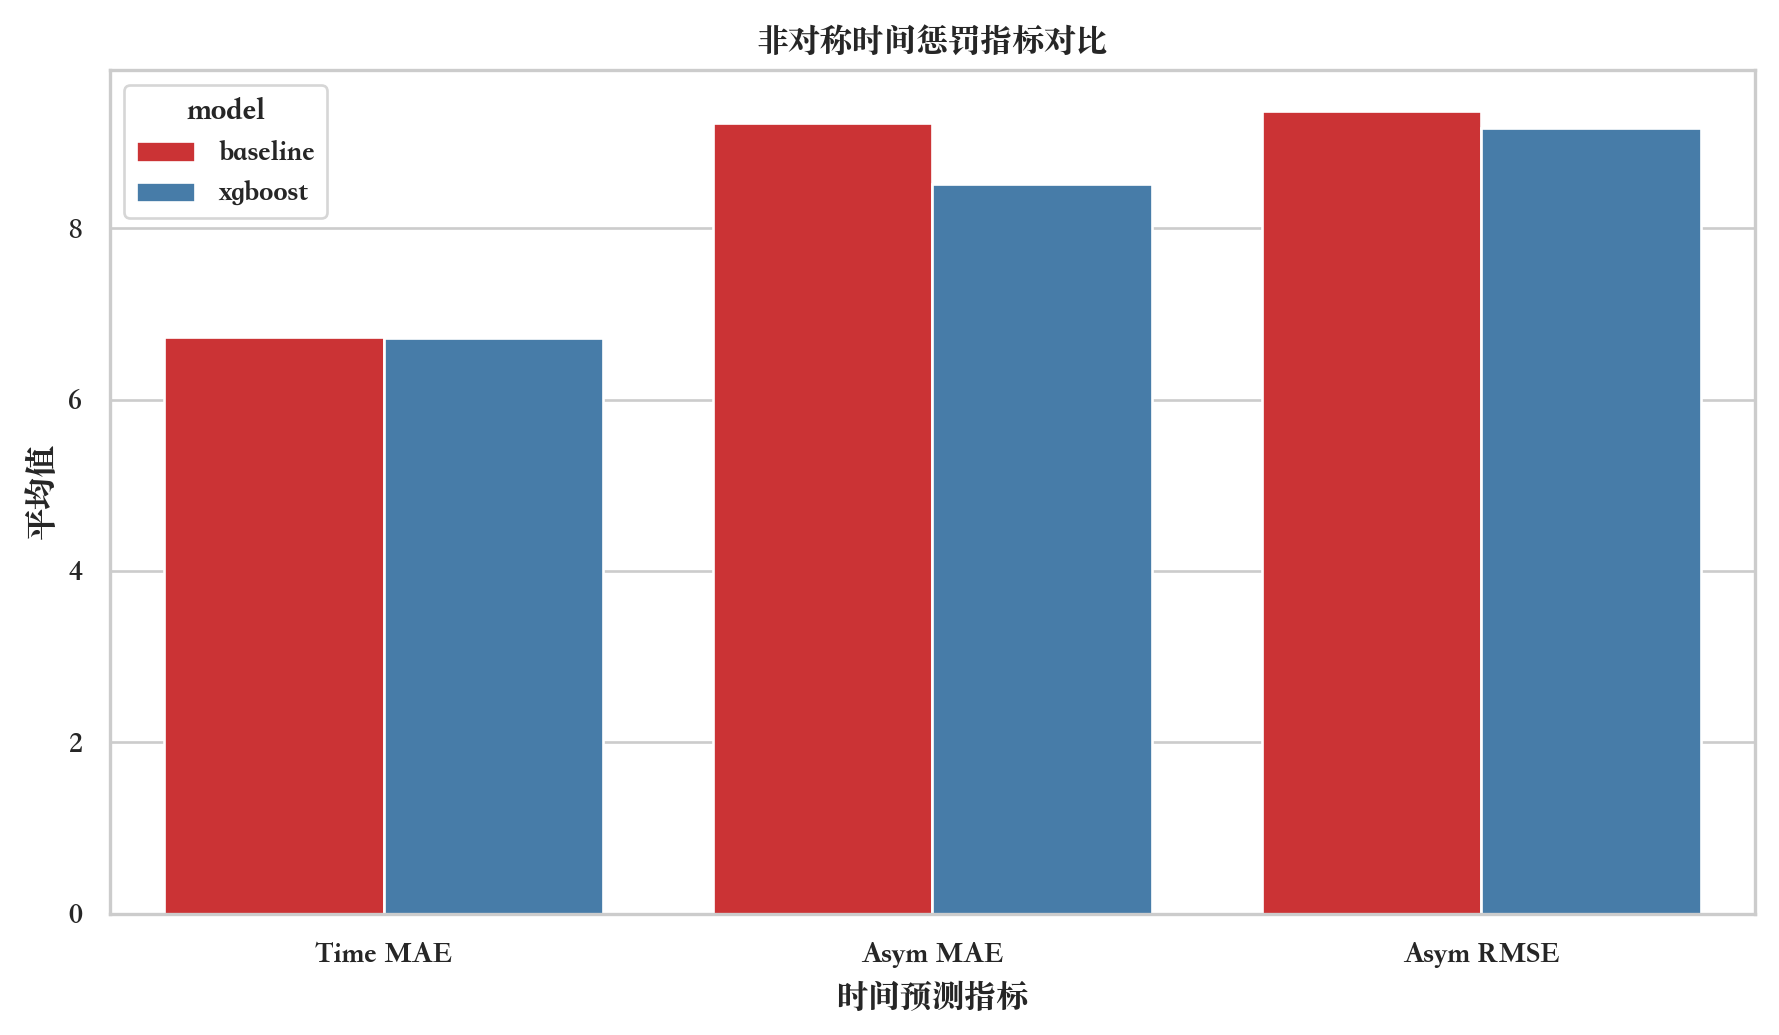
\includegraphics[width=\textwidth]{time_asymmetric_metrics.png}
    \caption{时间非对称指标}
  \end{subfigure}
  \caption{模型验证指标对比}
  \label{fig:cv_metrics}
\end{figure}

\section{OOF 融合}
模型融合基于 OOF 预测搜索线性权重。当前最优权重为 LightGBM 0.32、XGBoost 0.68，DL 和 GNN 默认权重为 0，表示稳定提交路径仅使用树模型。融合摘要见表\ref{tab:ensemble_summary}，权重可视化见图\ref{fig:ensemble_weights}。融合后 OOF 震级 RMSE 为 1.370，综合目标为 3.903。

\begin{table}[H]
  \centering
  \caption{融合权重与 OOF 指标}
  \label{tab:ensemble_summary}
  \begingroup
\footnotesize
\setlength{\tabcolsep}{4pt}
\begin{tabular}{lr}
\toprule
项目 & 数值 \\
\midrule
baseline & 0.12 \\
xgboost & 0.88 \\
dl & 0.00 \\
gnn & 0.00 \\
OOF Mag RMSE & 0.525 \\
OOF Time RMSE & 8.445 \\
OOF Ensemble Objective & 9.658 \\
\bottomrule
\end{tabular}
\endgroup

\end{table}

\begin{figure}[H]
  \centering
  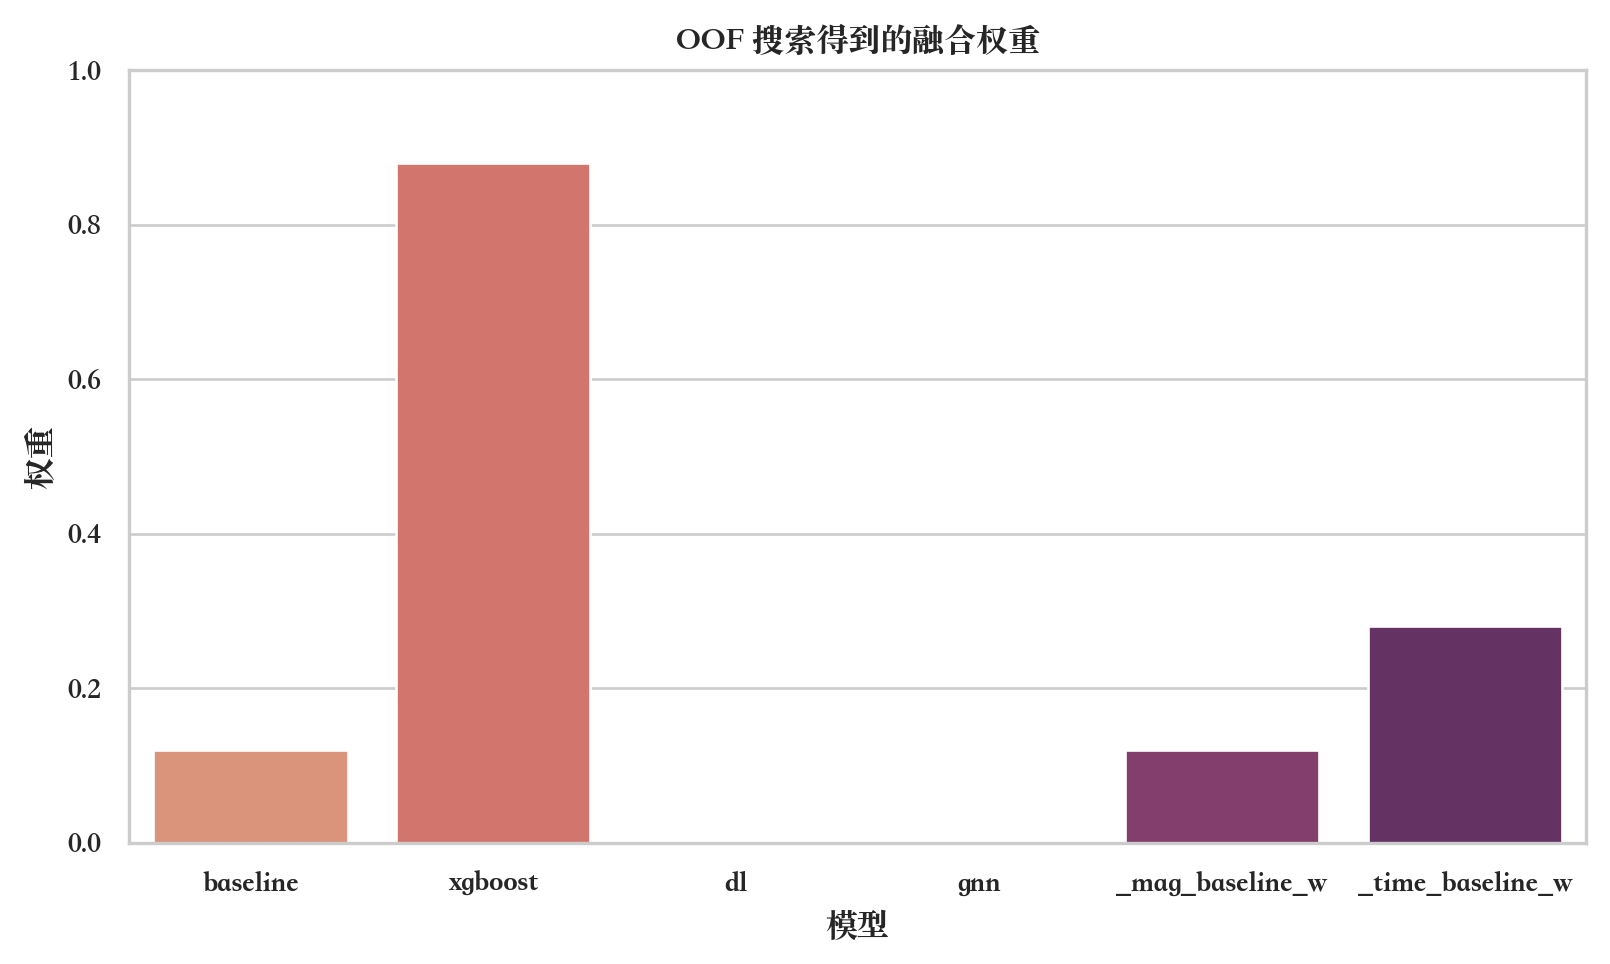
\includegraphics[width=0.65\textwidth]{ensemble_weights.png}
  \caption{OOF 融合权重}
  \label{fig:ensemble_weights}
\end{figure}

\section{测试序列提交结果}
20 条比赛验证序列的预测结果见表\ref{tab:submission_results}。最终提交文件包含 \texttt{mainshock\_id}、\texttt{predicted\_max\_mag}、\texttt{predicted\_time\_to\_max} 三列，预测时间均非负。图\ref{fig:submission_predictions}展示了预测震级和时间的分布，其中 2011 年日本东北地震序列的预测时间显著偏长，符合其大型俯冲带地震后余震持续活跃的直觉。

\begin{center}
\begingroup
\footnotesize
\setlength{\tabcolsep}{4pt}
\begin{longtable}{lrr}
\toprule
主震 ID & 预测最大余震 Mw & 预测时间差（天） \\
\midrule
\endfirsthead
\toprule
主震 ID & 预测最大余震 Mw & 预测时间差（天） \\
\midrule
\endhead
20010126031640\_eq & 4.700 & 0.390 \\
20021103221241\_eq & 4.900 & 0.165 \\
20031227160059\_eq & 6.770 & 5.145 \\
20041226005853\_eq & 6.100 & 0.249 \\
20070815234057\_eq & 5.000 & 1.310 \\
20080512062804\_eq & 5.000 & 0.953 \\
20100227080123\_eq & 4.400 & 0.356 \\
20110311054624\_eq & 6.466 & 18.346 \\
20120411083836\_eq & 5.600 & 0.608 \\
20130420000246\_eq & 4.000 & 0.728 \\
20150425061125\_eq & 4.800 & 0.565 \\
20190706031953\_eq & 4.100 & 0.276 \\
20201030115127\_eq & 4.000 & 0.081 \\
20210521134834\_eq & 3.400 & 1.109 \\
20210521180411\_eq & 4.400 & 0.769 \\
20210814122908\_eq & 4.200 & 0.341 \\
20220905045218\_eq & 3.800 & 0.212 \\
20230206011734\_eq & 4.800 & 0.776 \\
20231202143704\_eq & 4.600 & 1.825 \\
20240122180905\_eq & 4.100 & 0.386 \\
\bottomrule
\end{longtable}
\endgroup

\captionof{table}{20 条测试序列预测结果}
\label{tab:submission_results}
\end{center}

\begin{figure}[H]
  \centering
  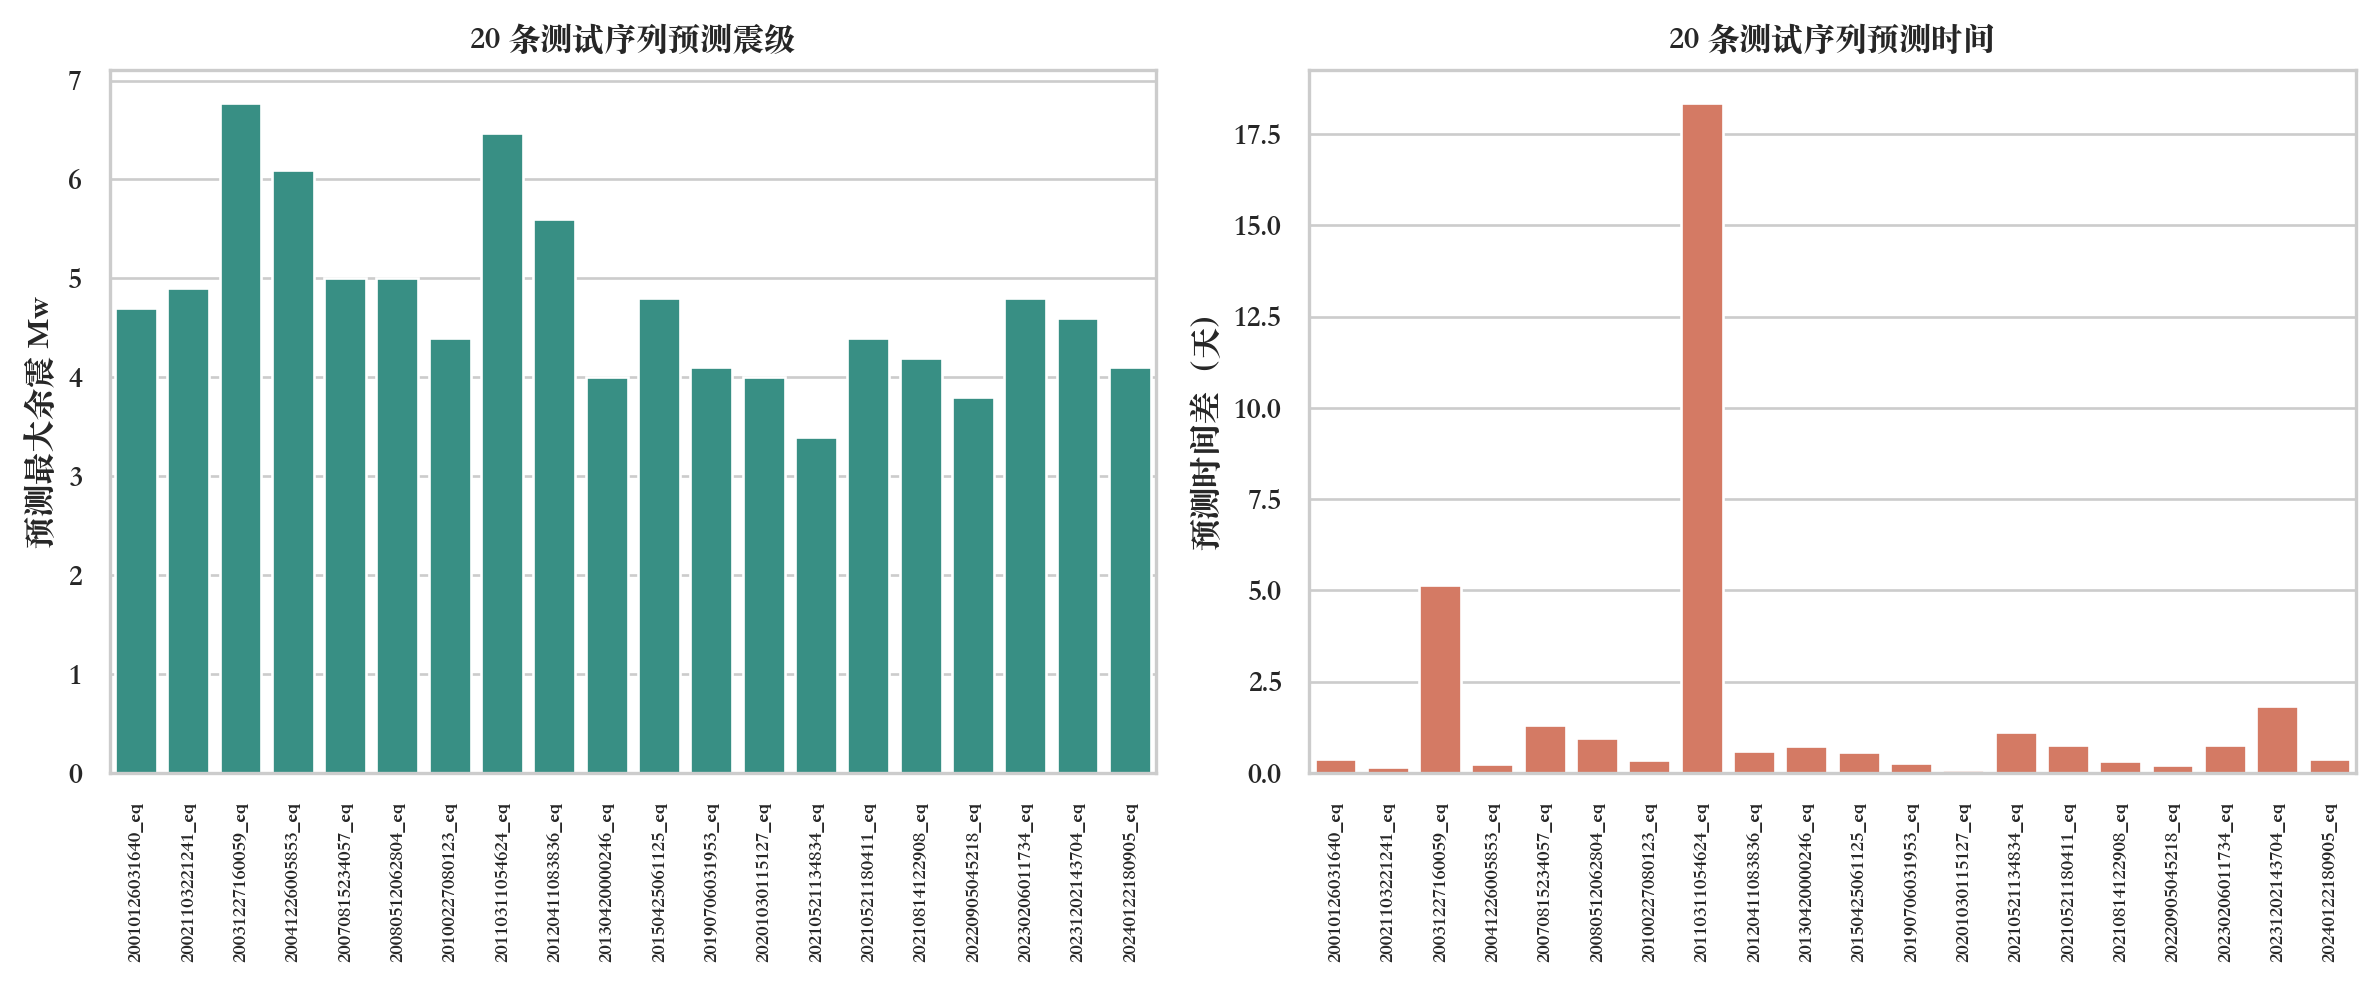
\includegraphics[width=0.96\textwidth]{submission_prediction_distribution.png}
  \caption{20 条测试序列预测分布}
  \label{fig:submission_predictions}
\end{figure}

\section{结果讨论}
从结果看，当前树模型已经形成稳健基线，但仍存在若干可解释现象。首先，目标变量零值比例高，导致总体 MAE 看似较低，但强余震样本的 RMSE 仍然决定模型上限。其次，G-R、Omori 和 ETAS 特征有效率受早期余震数量限制，在事件稀疏样本上依赖缺失值处理和 missing indicator。第三，GCMT 严格匹配带来高质量震源机制特征，但仍有 682 条样本未匹配，Unknown 类别本身也是模型需要学习的状态。最后，XGBoost 在时间指标上更稳定，可能与其正则化和树结构搜索方式有关，而 LightGBM 的非对称目标在震级维度保持较好表现。

\chapter{工程化复现与部署}

\section{项目模块}
项目结构已经按数据、特征、模型、训练、评估和推理分层，核心模块见表\ref{tab:module_structure}。

\begin{table}[H]
  \centering
  \caption{工程模块职责}
  \label{tab:module_structure}
  \begin{tabular}{p{0.28\textwidth}p{0.62\textwidth}}
\toprule
模块 & 职责 \\
\midrule
main.py & 统一命令入口，串联下载、序列、特征、训练和推理 \\
run.sh & 一键比赛流水线，支持跳过下载和可选 DL/GNN \\
src/data\_loader.py & 主震-余震序列构建与目标生成 \\
src/features.py & 地震学特征、板块边界、GCMT 震源机制融合 \\
src/models.py & LightGBM/XGBoost Baseline 与非对称目标 \\
src/dataset.py & 深度学习序列 Dataset、防泄漏预处理器 \\
src/models\_dl.py & Transformer 双输入融合模型 \\
src/models\_gnn.py & 有向时空因果 ST-GNN \\
scripts/make\_submission.py & 端到端单序列推理与提交格式化 \\
\bottomrule
\end{tabular}

\end{table}

\section{一键运行}
完整流程可通过 \texttt{run.sh} 执行。默认模式跳过深度模型，仅训练 LightGBM 与 XGBoost，适合快速稳定提交；若需要探索深度模型，可额外加入 \texttt{--with-dl} 或 \texttt{--with-gnn}。

\begin{lstlisting}[style=bashcode,caption={一键运行命令}]
./run.sh --skip-download
./run.sh --skip-download train-only
./run.sh --skip-download --with-dl train-only
./run.sh --skip-download --with-gnn train-only
\end{lstlisting}

推理脚本对单条测试序列执行实时特征提取、模型加载、融合预测和后处理裁剪。若深度模型权重大于 0 但产物缺失，脚本会跳过该模型并对剩余可用模型重新归一化权重；若所有模型均不可用，除非显式允许规则兜底，否则抛出错误，避免静默生成不可信结果。

\section{可复现性控制}
项目从以下层面控制可复现性：
\begin{enumerate}[label=\arabic*.]
  \item 固定随机种子，训练脚本记录 seed、模型参数和时间目标变换；
  \item 使用时间序列切分，不采用随机 K 折；
  \item 模型产物与特征列同步保存，推理按训练列补齐缺失特征；
  \item 深度学习预处理器保存为 joblib，推理复用训练时 scaler 和填充值；
  \item 输出 \texttt{model\_meta.json}、\texttt{feature\_cols.json}、\texttt{ensemble\_weights.json} 作为模型语义说明。
\end{enumerate}

\chapter{结论与展望}

本文构建了一套面向余震预测比赛的完整算法工程。特征工程方面，项目将 G-R、Omori、Båth's Law、生产率指数、空间各向异性、板块构造和 Global CMT 震源机制融合为 82 列高级特征；模型方面，使用 LightGBM 与 XGBoost 建立稳定树模型基线，并通过时间目标 log 变换、非对称时间惩罚和 OOF 融合增强预警语义；工程方面，实现了从数据构建到提交文件生成的一键流水线。

当前方案的主要优势在于稳健、可解释和可复现。地震学特征为模型提供物理先验，时间序列交叉验证避免未来信息泄漏，提交流水线能够处理单条新主震序列。局限也较明确：物理参数有效率仍受早期事件数限制，目标零膨胀尚未单独建模，深度模型目前以可选增强为主，尚未通过系统超参搜索充分发挥能力。

后续可从三方面继续提升。第一，引入更完整的区域低震级目录，提高 G-R、Omori 和 ETAS 参数覆盖率。第二，按俯冲带、走滑边界、板内地震和震源机制类型进行分层建模，减少全球模型的异质性压力。第三，对 Transformer 与 ST-GNN 进行 OOF 训练和权重搜索，使深度模型真正参与融合，而非仅作为接口储备。

\chapter*{参考文献}
\addcontentsline{toc}{chapter}{参考文献}

\begin{enumerate}[label={[\arabic*]}]
  \item Gutenberg, B., and Richter, C. F. Frequency of earthquakes in California. \textit{Bulletin of the Seismological Society of America}, 1944.
  \item Aki, K. Maximum likelihood estimate of b in the formula \(\log N=a-bM\) and its confidence limits. \textit{Bulletin of the Earthquake Research Institute}, 1965.
  \item Utsu, T. A statistical study on the occurrence of aftershocks. \textit{Geophysical Magazine}, 1961.
  \item Utsu, T., Ogata, Y., and Matsu'ura, R. S. The centenary of the Omori formula for a decay law of aftershock activity. \textit{Journal of Physics of the Earth}, 1995.
  \item Båth, M. Lateral inhomogeneities of the upper mantle. \textit{Tectonophysics}, 1965.
  \item Bird, P. An updated digital model of plate boundaries. \textit{Geochemistry, Geophysics, Geosystems}, 2003.
  \item Dziewonski, A. M., Chou, T. A., and Woodhouse, J. H. Determination of earthquake source parameters from waveform data for studies of global and regional seismicity. \textit{Journal of Geophysical Research}, 1981.
  \item Ke, G., Meng, Q., Finley, T., et al. LightGBM: A highly efficient gradient boosting decision tree. \textit{Advances in Neural Information Processing Systems}, 2017.
  \item Chen, T., and Guestrin, C. XGBoost: A scalable tree boosting system. \textit{Proceedings of the 22nd ACM SIGKDD}, 2016.
  \item Vaswani, A., Shazeer, N., Parmar, N., et al. Attention is all you need. \textit{Advances in Neural Information Processing Systems}, 2017.
\end{enumerate}

\appendix
\chapter{附录：关键命令与产物}

\section{报告资产生成}
\begin{lstlisting}[style=bashcode,caption={生成报告图表与表格}]
python scripts/build_report_assets.py
\end{lstlisting}

\section{LaTeX 编译}
\begin{lstlisting}[style=bashcode,caption={编译研究报告}]
cd reports/aftershock_research_report
latexmk -xelatex -interaction=nonstopmode aftershock_research_report.tex
\end{lstlisting}

\section{核心产物}
\begin{itemize}
  \item 高级特征表：\texttt{data/processed/advanced\_features.csv}
  \item 交叉验证指标：\texttt{data/models/cv\_metrics.csv}
  \item 模型元信息：\texttt{data/models/model\_meta.json}
  \item 融合权重：\texttt{data/models/ensemble\_weights.json}
  \item 提交文件：\texttt{data/processed/submission.csv}
\end{itemize}

\end{document}
